\chapter{Trabalhos Relacionados}\label{cap3}


Em Computação de Alto Desempenho é conhecido que, para um bom algoritmo paralelo executar, é preciso uma boa estratégia para a divisão da entrada e para a junção das várias soluções ao final. 

Há ainda a preocupação com a distribuição das tarefas entre os processadores, levando em conta que, ao final, todos eles devam ter realizado uma quantidade similar de processamento, evitando que alguns processadores fiquem ociosos enquanto outros estão sobrecarregados. Se isto acontecer, significa que a carga foi devidamente balanceada entre os processadores.

A geometria computacional é a área da computação que estuda soluções e estruturas de dados para problemas geométricos. O seu enfoque é buscar soluções sob o ponto de vista da análise de complexidade de algoritmos. Entre os problemas estudados estão a construção de fechos convexos, triangulações, ordenação de pontos espaciais, interseções de retas/planos, malhas e outros mais.

Neste capítulo, é apresentado inicialmente alguns conceitos necessários para um melhor entendimento dos trabalhos que estão sendo desenvolvidos nos últimos anos na área de particionamento de domínios para geração em paralelo de malha. Logo em seguida será apresentado os trabalhos relacionados a particionamento de domínios, dando ênfase no modo que é tratada a subdivisão dos domínios e a estimativa de carga em cada técnica apresentada. 


\section{Conceitos e Definições}\label{Geometria computacional}

\subsection{Geometria Computacional}\label{Geometria computacional}

A geometria computacional é a área da computação que estuda soluções e estruturas de dados para problemas geométricos. O seu enfoque é buscar soluções sob o ponto de vista da análise de complexidade de algoritmos. Entre os problemas estudados estão a construção de fechos convexos, triangulações, ordenação de pontos espaciais, interseções de retas/planos, malhas e outros mais.

\subsubsection{Fecho Convexo}

O fecho convexo de um conjunto finito de pontos é o menor conjunto convexo que contém tais pontos. Segundo \cite{bib:Carvalho91} um conjunto $K$ do $\Re^{n}$, sendo $n$ um inteiro não negativo, é convexo se quaisquer que sejam  $x \in K$, $y \in K$ e $0 \leq \lambda \leq 1$, $\lambda \in \Re$ , tem-se $\lambda x + (1-\lambda)y \in K $. Ou seja, todas as combinações convexas dos elementos de $K$ pertencem a $K$. Um ponto $p$ é dito ser combinação convexa dos pontos $p_{i} \in K$  se $p = \displaystyle\sum_{i=1}^{|K|} p_{i}\lambda_i $, sendo $ \displaystyle\sum_{i=1}^{|K|} \lambda_i = 1 $.

Um ponto $w \in K$ é um ponto extremo de $K$ se não pode ser conectado a um elemento de $K$ por um segmento de reta aberto pertencente a $K$. O fecho convexo de um conjunto finito $C$ de pontos no $\Re^{n}$, sendo $n$ um inteiro não negativo, é o conjunto de todas as combinações convexas de elementos de $C$. Em outras palavras pode-se dizer que o fecho convexo é um conjunto finito de pontos com menor área geométrica que engloba todos os pontos do conjunto (Figura \ref{fig:fecho convexo}).

 \begin{figure}[htbp]
     \centering
     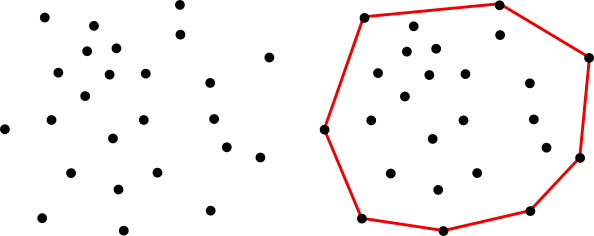
\includegraphics[width=0.5\textwidth]{fig/fecho_convexo.png}
     \caption{Conjunto de pontos e o seu fecho convexo.} 
     \label{fig:fecho convexo}
 \end{figure}

\subsubsection{Ponto de Steiner}

No triângulo ABC, sejam:
\begin{itemize}
  \item A’ o simétrico de A em relação a G
  \item B’ o simétrico de B em relação a G
  \item C’ o simétrico de C em relação a G;
\end{itemize}

As três circunferências definidas pelos conjuntos de ternos de pontos AB’C’, BA’C’, CA’B’ intersectam-se num ponto do circuncírculo - ponto de Steiner. A cada uma das três circunferências dá-se o nome de “círculo de Steiner”, como mostra a figura \ref{fig:steiner}.

 \begin{figure}[htbp]
     \centering
     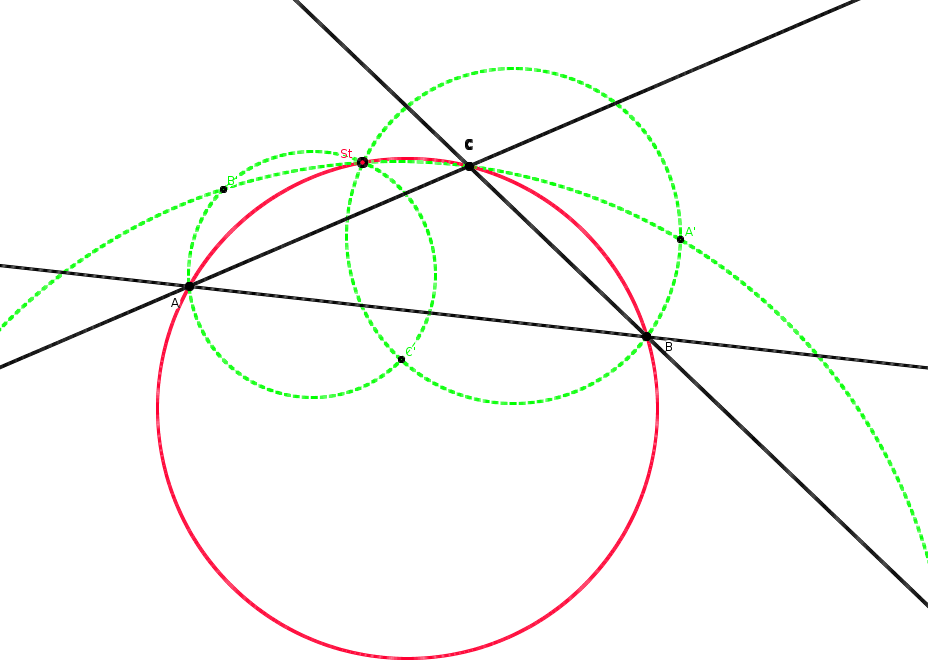
\includegraphics[width=0.8\textwidth]{fig/steiner.png}
     \caption{Ponto de Steiner para um triângulo ABC.} 
     \label{fig:steiner}
 \end{figure}

\subsubsection{Triangulação e Malha}

Triangulações são muitas vezes chamadas de malhas ou usadas como malhas, como no caso do método dos elementos finitos (MEF), já que malha é uma união de elementos, que podem ser triângulos, por exemplo. Pode-se definir uma malha $M$ de uma maneira genérica como:

\begin{itemize}
 \item $\varOmega = \bigcup\limits_{k \in M} k $, onde $\varOmega$ é um domínio finito limitado,
 \item O interior de cada elemento $k$ em $M$ é não vazio,
 \item A interseção do interior de dois elementos de $M$ é vazia.
\end{itemize}

Uma triangulação também é uma malha, mas nem toda malha é uma triangulação. Neste trabalho quando for mencionado malha, será sempre a malha que respeita as mesmas propriedades de uma triangulação. A definição de triangulação segundo \cite{bib:Triangulations_applications} diz que:

\begin{itemize}
  \item Nenhum triângulo pertencente à triangulação pode ter pontos colineares.
  \item A interseção do interior de quaisquer dois triângulos pertencentes à triangulação é vazia.
  \item As bordas de 2 triângulos quaisquer só podem fazer interseção com vértices ou arestas.
  \item A união de todos os triângulos da triangulação é igual ao domínio.  
  \item O domínio deve ser conectado.
  \item Não deve existir buracos na triangulação, a menos que eles sejam definidos como entrada.
  \item Se um triângulo está na borda da triangulação então ele faz interseção por aresta no máximo dois triângulos.
\end{itemize}


Existem malhas de diferentes geometrias e dimensões. Caso a topologia de elementos e vértices da malha siga alguma regra simples de indexação, essa malha será definida como estruturada, caso contrário, ela é definida como não-estruturada. Nas malhas estruturadas o conhecimento dos vizinhos de cada elemento não depende do armazenamento ou existência desta informação. Já nas não-estruturadas, para se ter conhecimento dos vizinhos, é necessário armazenar ou calcular estas informações. Existem ainda as malhas mistas, que combinam malhas estruturadas e não-estruturadas (Figura \ref{fig:est_e_n_est}).

As malhas também podem ser classificadas de acordo com a geometria dos seus elementos, já que não são necessariamente formadas somente de triângulos.. Para malhas bidimensionais, por exemplo, elas podem ser de elementos triangulares ou quadrilaterais, por exemplo, como mostra a Figura \ref{fig:est_e_n_est}.

 \begin{figure}[htbp]
     \centering
     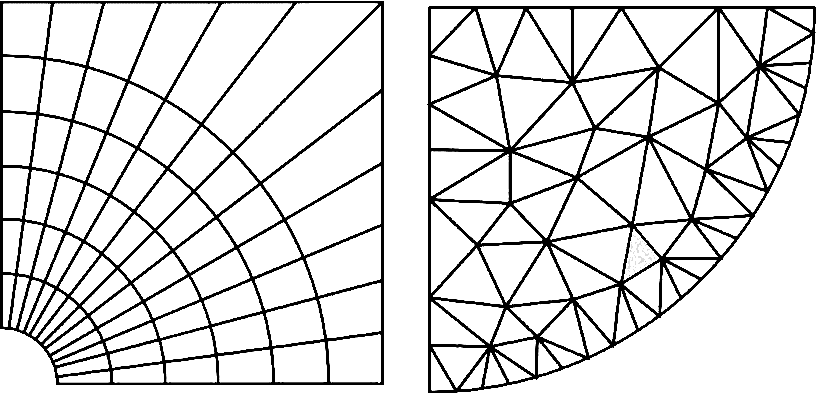
\includegraphics[width=0.5\textwidth]{fig/est_e_n_est.png}
     \caption{Exemplo de malha quadrilateral estruturada e não-estruturada triangular.} 
     \label{fig:est_e_n_est}
 \end{figure}
 
Para muitas aplicações, a qualidade dos elementos da malha é muito importante. Para classificar um elemento de uma malha triangular como bom ou ruim pode-se utilizar, dentre outras, uma métrica que é definida como $ \alpha = 2R_i / R_c $, onde $R_i$ e $R_c$ são os raios dos círculos inscrito e circunscrito, respectivamente. 
 
Esta métrica $\alpha$ tem valor $1,0$ para um triângulo equilátero. Quanto pior a qualidade do elemento, mais próximo de $0,0$ é o valor de $\alpha$. Pode-se dizer que os elementos com $\alpha \leq 0,1$ são de péssima qualidade e que os elementos com $\alpha \geq 0,7$ são de boa qualidade, como mostra a Figura \ref{fig:qualidade_elemento}.

 \begin{figure}[htbp]
     \centering
     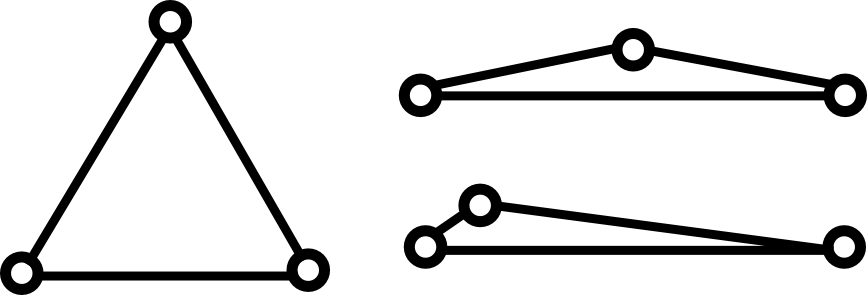
\includegraphics[width=0.5\textwidth]{fig/qualidade_elemento.png}
     \caption{Exemplo de um elemento triangular de boa qualidade (esquerda) e dois de péssima qualidade (direita).} 
     \label{fig:qualidade_elemento}
 \end{figure}

\subsection{Geração de Malha}\label{Geração de Malha}

Nesta seção, são apresentadas as técnicas de geração de malhas triangulares mais conhecidas atualmente. Existem diversos algoritmos para geração de malhas, porém eles podem ser enquadrados uma das categorias a seguir:

\begin{itemize}
  \item Avanço de fronteira, técnica em que a malha é gerada a partir da borda da região;

  \item Delaunay, técnica em que a malha é gerada procurando-se maximizar o menor ângulo dos triângulos gerados para um dado conjunto de pontos;

  \item Arbitrária, técnica em que a malha é gerada de maneira diferente das anteriores.
\end{itemize}

\subsubsection{Avanço de Fronteira}

Este é um dos métodos mais populares de geração de malhas e consiste em criar os elementos no interior do domínio progressivamente a partir de um contorno, especificando a região a ser preenchida (Figura~\ref{fig:AF}a). Este contorno é chamado de fronteira inicial ou borda. Os elementos são gerados a partir dessa fronteira dada como entrada. Uma fronteira bidimensional é formada por um conjunto de arestas.

À medida que o algoritmo progride, a fronteira avança em direção ao interior, sempre removendo ou adicionando elementos de fronteira até que todo o domínio seja preenchido. O algoritmo chega ao fim quando não há mais fronteira, ou seja, o domínio foi totalmente triangularizado. 

Há casos em que o algoritmo não consegue mais gerar elementos para uma determinada fronteira, isso indica que o algoritmo falhou. O caso de falha ocorre quando todos os possíveis elementos a serem criados se sobrepõem a um elemento já existente. Por isso, é importante verificar se elementos se interceptam. Os casos de falha geralmente acontecem em modelos tridimensionais. Entretanto, já existem técnicas para contornar esses problemas e gerar malhas em modelos que falhariam.

Para gerar os novos triângulos no interior do domínio, é necessário criar novos pontos que não pertencem aos dados de entrada. Em geral, são utilizados os pontos de Steiner para isso \cite{bib:Ruppert99}.

Um algoritmo de avanço de fronteira procede da seguinte maneira no caso 2D (Figura~\ref{fig:AF}):
 
 \begin{enumerate}
\item{ Selecione uma aresta da fronteira, a aresta base (fig.~\ref{fig:AF}b);}
\item{ Encontre um ponto ideal para a formação de um novo triângulo com a aresta base (fig.~\ref{fig:AF}c);}
\item{ Crie uma região de busca em torno desse ponto ideal (fig.~\ref{fig:AF}d);}
\item{ Selecione o ponto dentro dessa região de busca cujo triângulo (entre esse ponto e a aresta base) seja válido e seja o de melhor qualidade, que pode ser um novo ponto ou um ponto já pertencente à malha;}
\item{ Forme o novo triângulo com o ponto selecionado e adicione-o à malha (fig.~\ref{fig:AF}e);}
\item{ Atualize a fronteira, inserindo as arestas que foram criadas e removendo as arestas que já existiam;}
\item{ Se existir aresta na fronteira, volte para o passo 1.}
\end{enumerate}

 \begin{figure}[htbp]
     \centering
     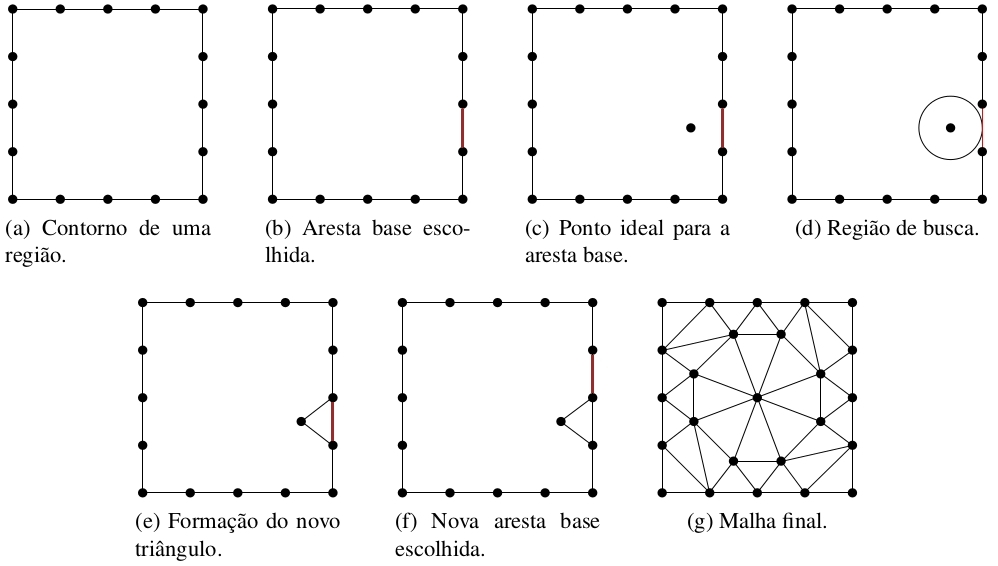
\includegraphics[width=1\textwidth]{fig/AF.jpg}
     \caption{Avanço de fronteira \cite{bib:Freitas10}.} 
     \label{fig:AF}
 \end{figure}

Pelo fato da fronteira ser sempre respeitada, os algoritmos de avanço de fronteira têm facilidade em tratar regiões descontínuas, ou por conterem buracos, ou por serem regiões separadas. Como os elementos mais próximos da borda são gerados primeiro, em geral, eles têm uma boa qualidade. A boa qualidade da malha gerada provê estabilidade e precisão à aplicação de métodos numéricos (como os métodos dos elementos finitos).

Porém, nem sempre todos os elementos gerados têm boa qualidade. Ao contrário dos elementos mais próximos da borda, os elementos mais internos à malha nem sempre têm boa qualidade devido à região tornar-se menor à medida que a fronteira avança. Geralmente uma técnica de suavização ou otimização é aplicada na malha resultante do algoritmo para tratar esses casos.

\subsubsection{Delaunay}

Esta é uma técnica bastante conhecida na área de geração de malhas, cujo nome é uma homenagem ao matemático russo Boris Delaunay. A entrada para esse problema é um conjunto de pontos e, geralmente, não são utilizados os pontos de Steiner para formar os triângulos.

O critério de Delaunay para a formação dos triângulos é que não exista nenhum outro ponto dentro do círculo que passa pelos três pontos desse triângulo (seu circuncírculo), critério este também chamado de "esfera vazia" (o circuncírculo desse triângulo, Figura~\ref{fig:criterio_delaunay}). O critério de Delaunay em si não se constitui num método de geração de malhas, mas é uma forma de saber onde os pontos devem estar localizados no espaço.

 \begin{figure}[htbp]
     \centering
     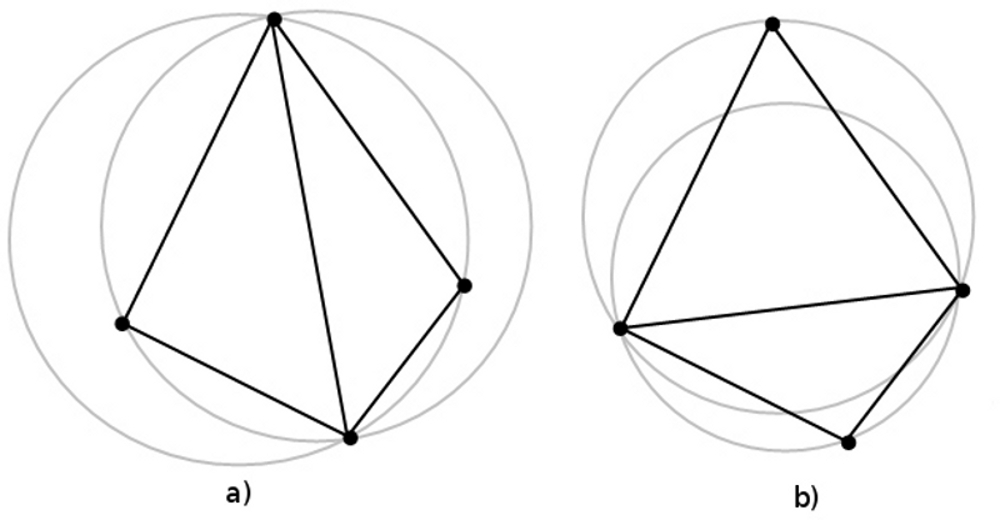
\includegraphics[width=0.65\textwidth]{fig/criterio_delaunay.jpg}
     \caption{a) Critério de Delaunay falhando para os dois triângulos. b) Triangulação válida respeitando o critério de Delaunay.} 
     \label{fig:criterio_delaunay}
 \end{figure}

A malha gerada por Delaunay visa maximizar os ângulos internos dos triângulos gerados, ou seja, dada uma aresta da triangulação de Delaunay, o ponto que forma o maior ângulo com essa aresta é o ponto que formará um triângulo de Delaunay com ela.

Existem algumas variações de algoritmos de Delaunay. Em uma delas, encontra-se uma aresta que faz parte da triangulação que é, em geral, uma aresta pertencente ao fecho convexo. A partir dela, é encontrado o ponto que formará um triângulo de Delaunay. Assim, com as novas arestas, encontram-se novos triângulos, em um algoritmo parecido com o de avanço de fronteira. Uma outra variação é feita a partir de inserção de pontos. A entrada é uma malha triangular não necessariamente de Delaunay e se modifica essa malha (de apenas um subconjunto de pontos da entrada) pré-existente (Figura~\ref{fig:triangulacao_insercao}).

\begin{figure}[htbp]
     \centering
     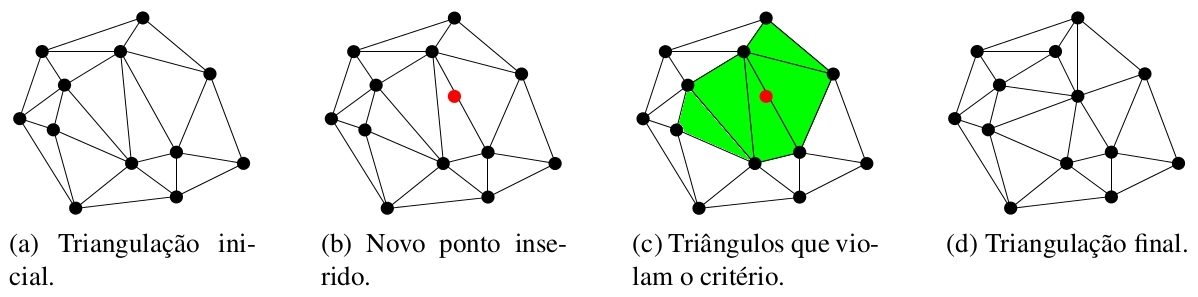
\includegraphics[width=1\textwidth]{fig/triangulacao_insercao.jpg}
     \caption{Triangulação por inserção de pontos \cite{bib:Freitas10}.} 
     \label{fig:triangulacao_insercao}
 \end{figure}

 Dependendo da disposição dos pontos da entrada, a triangulação final pode não ter boa qualidade, principalmente em regiões críticas, próximas à borda, gerando instabilidade em métodos numéricos. Uma alternativa para melhorar essa malha é fazer refinamentos e otimizações, que fazem uso de pontos de Steiner.

\subsubsection{Arbitrária}

As técnicas de geração de malha arbitrárias são aquelas que não se enquadram nem como Avanço de Fronteira e nem como Delaunay. As malhas são geradas em geral por algoritmos de varredura ou algum outro método.

Outro uso que essas malhas possuem é nas demonstrações de teoremas. O problema de ordenação de pontos pode ser reduzido ao problema de geração de malhas bidimensionais \cite{bib:Carvalho91}. Prova-se por redução que pode ser gerada uma malha triangular a partir do fecho convexo de um conjunto de pontos em duas dimensões numa complexidade na ordem de $O (n \log n)$.

\subsection{Geração de Malha em Paralelo}\label{Geração de Malha em Paralelo}

Na geração em paralelo é necessário dividir a entrada para realizar o processamento em paralelo das diversas partes. Existem duas formas de decompor o domínio. Na primeira forma, uma malha grosseira da região é rapidamente gerada, sequencialmente, e dividida entre os processadores. Essa forma, chamada de decomposição discreta do domínio, envolve ainda o problema de particionamento da malha. A segunda forma de decompor o domínio envolve dividir a região a partir de funções, segmentos, eixos inerciais, ou estruturas auxiliares, por isso chamada de decomposição contínua do domínio. Cada subdomínio é enviado a um processador, onde a malha será gerada.

Uma malha de interface é um conjunto de segmentos ou triângulos para o caso bidimensional ou, no caso tridimensional, um conjunto de triângulos ou tetraedros. Essa malha de interface faz a conexão entre duas partições vizinhas e faz o papel de uma nova fronteira. A forma que ela é criada vai depender da técnica que está sendo utilizada para particionar o domínio.

O particionamento contínuo pode ainda, ser subdividido em duas categorias, dependendo da forma como é gerada a malha entre os subdomínios, chamada de malha de interface. Se essa malha for gerada antes da malha interna ao subdomínio, essa abordagem é chamada de \textit{a priori}. Caso ela seja gerada depois, é chamada de \textit{a posteriori}. A geração da malha de interface \textit{a posteriori} geralmente requer sincronização entre processos. No trabalho de \cite{bib:deCougny99} apresenta esta classificação.

Existe outra classificação apresentada por \cite{bib:Survey_Chrisochoides05} que classifica as técnicas de acordo com a maneira que o domínio é decomposto. Podemos ter então técnicas classificadas como Discretas ou Contínuas. 

As técnicas de decomposição Discreta geralmente utilizam uma malha grosseira baseada na entrada dada. Primeiramente são definidas as regiões e em seguida as bordas destas regiões são refinadas (tanto as interfaces entre dois subdomínios quanto o contorno dado como entrada). Após isto as regiões, também chamadas de sub-malhas,  estarão prontas para a geração da malha.

Já as técnicas de decomposição Contínua não utilizam um malha grosseira. As regiões criadas serão compostas por parte do contorno de entrada juntamente com uma parte da região interna, criando assim subdomínios. A região interna pode necessitar da criação de uma interface antes da geração da malha (\textit{a priori}), assim como pode ser gerada depois (\textit{a posteriori}). Uma vantagem da decomposição Contínua em relação a Discreta é que a entrada não é modificada.

\subsection{Computação de Alto Desempenho}\label{Computação de alto desempenho}

Computação de Alto Desempenho ou HPC (do inglês \textit{High-performance computing}) se refere ao uso de \textit{clusters} ou supercomputadores em tarefas que requerem grandes recursos de computação. O uso eficiente desses recursos é o principal foco de estudo nessa área. \textit{Cluster} é um conjunto de computadores de alto desempenho interconectados por uma rede local que trabalham em conjunto como um único recurso de processamento.

\subsubsection{Modelos de Arquiteturas}

Em programas que executam sequencialmente não existe a preocupação que uma dada posição de memória seja alterada no mesmo tempo que ela esteja sendo lida. Em computação paralela há essa preocupação e existem várias técnicas para manter a ordem de leitura e escrita na memória. Basicamente há dois tipos de arquiteturas (Figura \ref{fig:arquiteturas}):

  \begin{itemize}
    \item Memória Compartilhada

    Engloba basicamente os sistemas UMA (Uniform Memory Acess), ou seja, o acesso à memória é feito de forma uniforme através de endereçamento direto. Assim, todos os processadores de um computador compartilham um mesmo espaço de memória e para isso deve haver um controle na leitura e escrita na memória.

    \item Memória Distribuída
    
    Cada um dos processadores têm acesso a um espaço único de endereçamento de memória privada. Cada módulo da memória pode ser acessado diretamente por apenas um dos processadores. A comunicação entre os processos ocorre através de troca de mensagens.   
  \end{itemize}

   \begin{figure}[htbp]
     \centering
     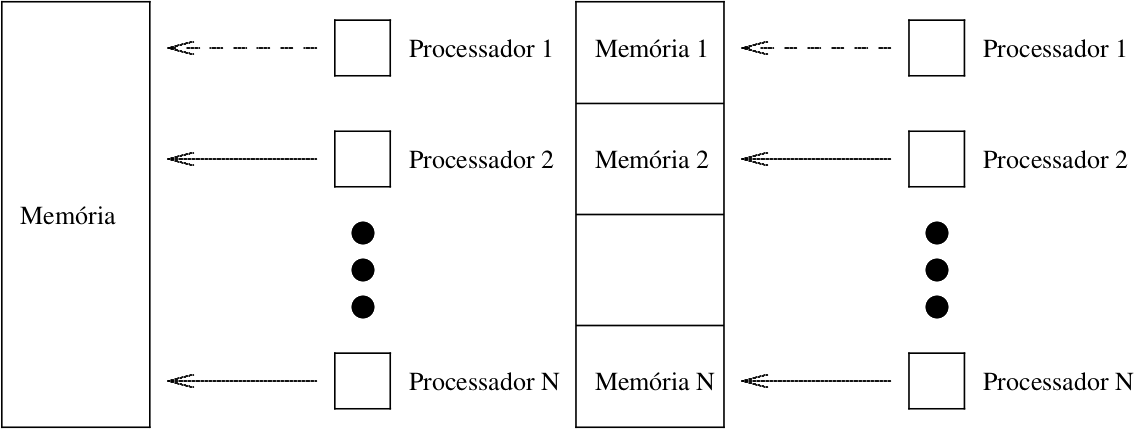
\includegraphics[width=1.0\textwidth]{fig/arquiteturas.png}
     \caption{Estratégia de balanceamento não-centralizado onde todos os nós podem se comunicar entre si. Memória compartilhada à esquerda e memória distribuída à direita.} 
     \label{fig:arquiteturas}
 \end{figure}

\subsubsection{Balanceamento de Carga}\label{Balanceamento de carga}

Uma aplicação que executa em paralelo cria várias novas tarefas que devem ser distribuídas entre os processadores existentes. Quando a quantidade de tarefas se torna maior que a quantidade de processadores disponíveis, torna-se necessário um balanceamento de carga, ou seja,  distribuir o processamento entre os processadores de modo a obter a maior velocidade possível de execução. O principal objetivo é manter os processadores ocupados a maior parte do tempo possível evitando que alguns deles fiquem ociosos enquanto outros estão executando alguma tarefa. 

Esse balanceamento pode ser estático (o balanceamento ocorre antes da execução de qualquer processo) ou dinâmico (é realizado durante a execução do processo). O principal problema de um balanceamento estático é a dificuldade em estimar com precisão os tempos de execução das várias partes do programa. O modelo de balanceamento dinâmico possui duas classificações:

  \begin{figure}[htbp]
     \centering
     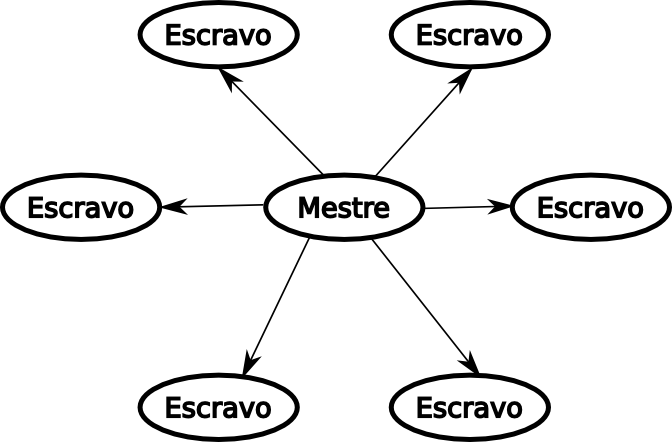
\includegraphics[width=0.5\textwidth]{fig/mestre_escravo.png}
     \caption{Estratégia de balanceamento centralizado mestre/escravo onde um processo controla todas as tarefas e os escravos solicitam e executam as mesmas.} 
     \label{fig:mestre_escravo}
 \end{figure}

\begin{enumerate}
 \item Centralizado (Figura \ref{fig:mestre_escravo})
    \begin{itemize}
      \item Todas as tarefas são manipuladas a partir de uma localização central.
      \item Exemplo: Modelo mestre-escravo - o processo mestre mantém a coleção de tarefas a serem executadas e os processos escravos solicitam tarefas.
    \end{itemize}
 
    \item Não-centralizado  (Figura \ref{fig:pulling})
    \begin{itemize}
      \item Uma coleção de processos trabalhadores opera sobre um problema, e esses trabalhadores interagem entre si, reportando o resultado final a um único processo.
      \item Exemplo: Algoritmo de \textit{polling} aleatório - o processo $P_i$ pede tarefas ao processo $P_x$, onde $x$ é um número selecionado aleatoriamente entre $0$ e $n-1$ (excluindo $i$).
    \end{itemize} 
\end{enumerate}

 \begin{figure}[htbp]
     \centering
     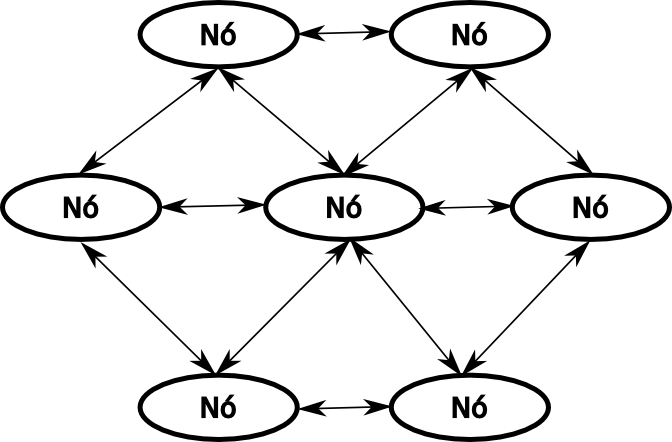
\includegraphics[width=0.5\textwidth]{fig/pulling.png}
     \caption{Estratégia de balanceamento não-centralizado onde os nós podem se comunicar entre si.} 
     \label{fig:pulling}
 \end{figure}

\subsubsection{Métricas de Desempenho}\label{Metricas de desempenho}

Ao utilizar uma aplicação paralela, surge o interesse em saber o ganho de velocidade quando comparado a uma aplicação sequencial. Para isso existem algumas métricas utilizadas:

\begin{itemize}
 \item Escalabilidade

 É a propriedade de um sistema que lhe confere a capacidade de aumentar seu desempenho sob uma determinada carga, quando mais recursos (processadores) são acrescentados a esse sistema. Ou seja, pode-se falar que um algoritmo é escalável se ele pode ser utilizado em uma grande quantidade de processadores sem que aconteça uma queda em sua velocidade.
 
 Pode-se dizer que um sistema é escalável quando ele resolve um problema de magnitude $\gamma$ com um recurso $R$, e consegue resolver um problema de magnitude $n\gamma$ com um recurso $nR$. Ou seja, sempre que aumentar os recursos computacionais, aumentará proporcionalmente a capacidade de resolver problemas maiores.
 
 \item \textit{Speed-up}

  Esta métrica mostra quantas vezes um programa paralelo é mais rápido que um serial. Para obter um \textit{speed-up} linear tem-se que obter um programa com tempo de execução $x$ vezes mais rápido quando aumentado em $x$ o número de processadores. Já um \textit{speed-up} super linear seria obter um ganho maior que $x$ quando aumentado em $x$ o número de processadores.
 
 O \textit{speed-up} $S$ para $p$ processadores é calculado pela seguinte formula: $ S(p) = T_s / T_p $, onde $T_s$ é o tempo de execução do programa sequencialmente e $T_p$ é o tempo do programa executando em paralelo para $p$ processadores.
 
 Na prática um \textit{speed-up} linear é difícil de se obter. À medida que a quantidade de processadores aumentam, a comunicação entre os processos aumenta e isso faz o tempo de execução cair, derrubando assim o \textit{speed-up}.
 
\end{itemize}


\subsection{Estrutura de Dados}\label{Estrutura de dados}

Diversas estruturas de dados que foram criadas na área da computação são muito usadas em problemas de computação gráfica. No contexto desse trabalho, essas estruturas têm o objetivo de fazer uma decomposição espacial do domínio. Com essas decomposições, diversos cálculos são otimizados fazendo uma busca em qual parte da decomposição o objeto de interesse está e limitando os cálculos apenas aos elementos que pertencem a essa decomposição.

Essas estruturas são utilizadas em diversas aplicações como tratamento de colisão e renderização (Figura \ref{fig:ex_decomposicao}). Entre as estruturas de dados bidimensionais, as mais importantes são a \textit{quadtree}, \textit{octree} e a \textit{binary space partitioning} ou simplesmente BSP.

 \begin{figure}[htbp]
     \centering
     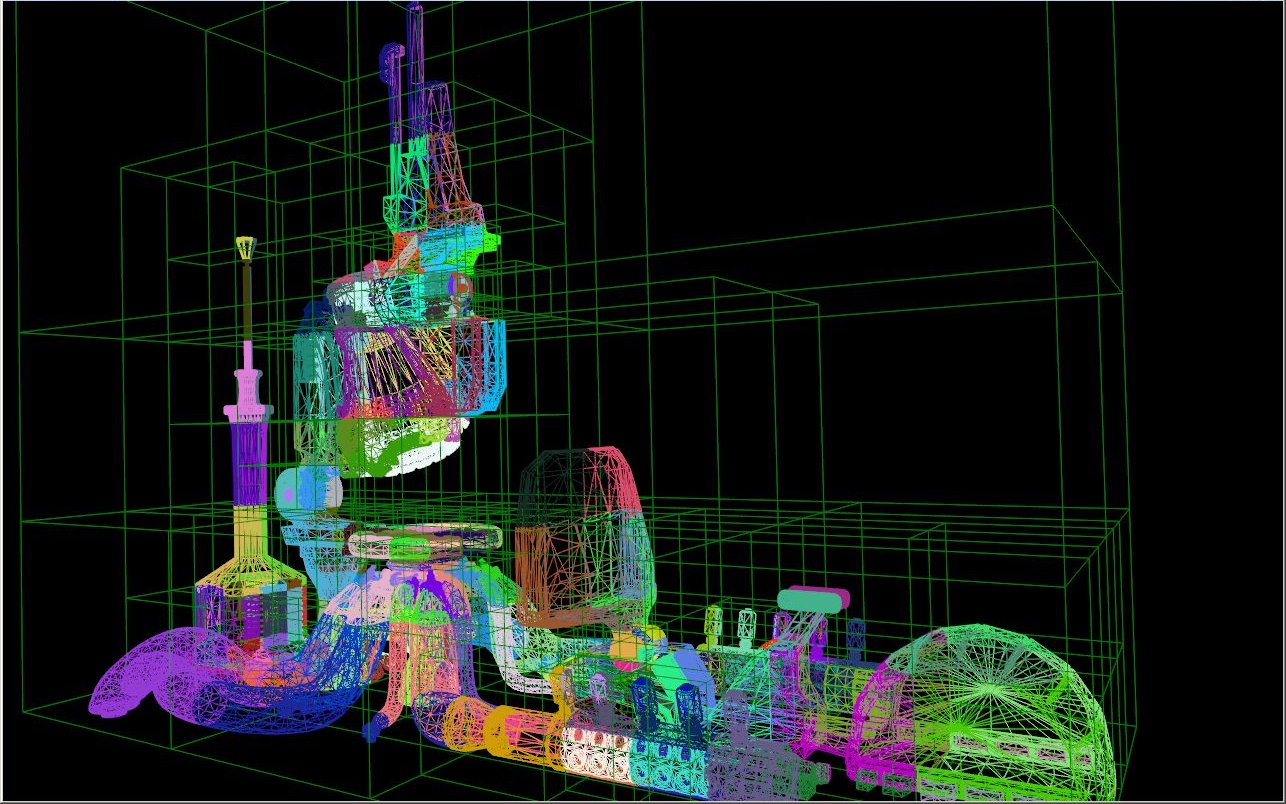
\includegraphics[width=0.7\textwidth]{fig/ex_decomposicao.jpg}
     \caption{Exemplo de uma decomposição espacial feita para renderização e teste de colisão. Fonte: http://togeskov.net/} 
     \label{fig:ex_decomposicao}
 \end{figure}

\subsubsection{\textit{Quadtree}}

Uma \textit{quadtree} é uma estrutura de dados baseada em árvore em que cada nó possui exatamente quatro filhos (Figura \ref{fig:quadtree_tree}). Em geral \textit{quadtrees} são utilizadas para decompor domínios bidimensionais recursivamente em quatro regiões de mesmo tamanho. As \textit{quadtrees} podem ser classificadas de acordo com o tipo do dado que elas representam (regiões, pontos, arestas, polígonos), isso vai depender do tipo de aplicação para o qual ele está sendo utilizada. Essa classificação altera o critério de subdivisão da \textit{quadtree}, por exemplo, o critério pode ser a quantidade de pontos internos há um quadrante da \textit{quadtree}, com isto é garantido a quantidade máxima de pontos internos a cada célula desta \textit{quadtree}.

 \begin{figure}[htbp]
     \centering
     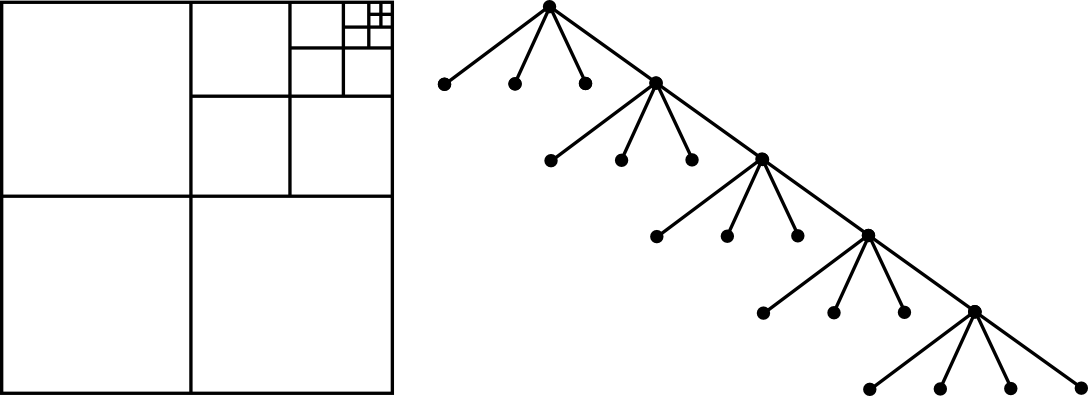
\includegraphics[width=0.8\textwidth]{fig/quadtree_tree.png}
     \caption{Uma subdivisão feita por \textit{quadtree} com cinco níveis e sua representação em árvore.} 
     \label{fig:quadtree_tree}
 \end{figure}

\subsubsection{\textit{Octree}} 

A \textit{octree} é a versão tridimensional da \textit{quadtree}, por isso as mesmas propriedades da \textit{quadtree}se aplicam a ela (Figura \ref{fig:octree_tree}). A diferença é que a entrada será divida sempre em 8 partes com regiões de mesmo tamanho. Os cortes serão realizados nos eixos X, Y e Z.	


 \begin{figure}[htbp]
     \centering
     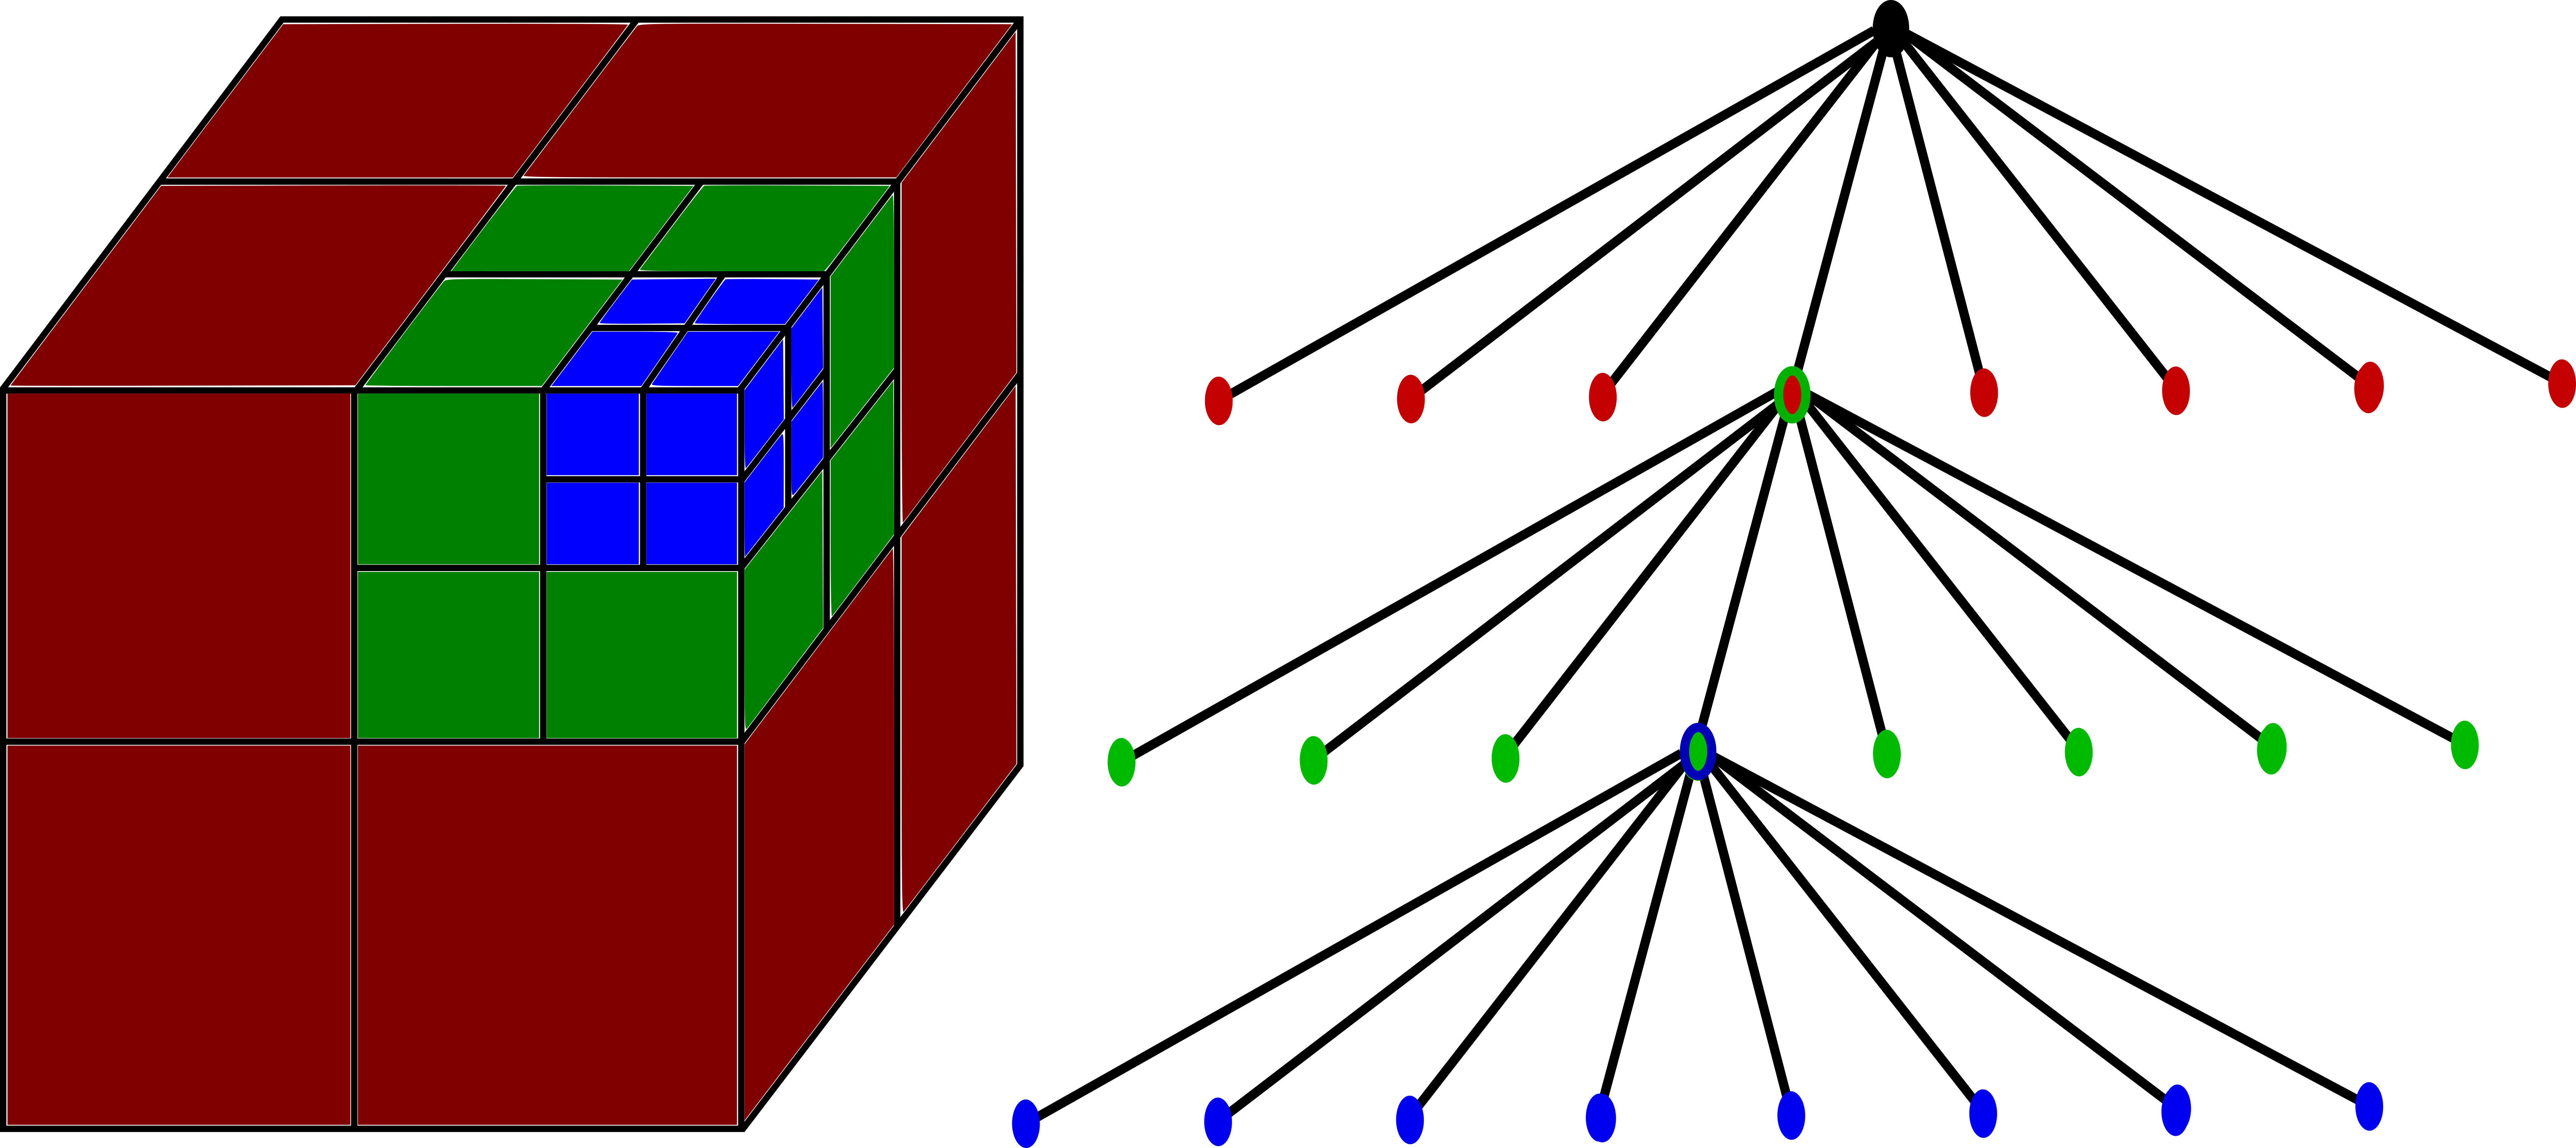
\includegraphics[width=0.8\textwidth]{fig/octree_tree.png}
     \caption{Uma subdivisão feita por \textit{octree} com três níveis e sua representação em árvore.} 
     \label{fig:octree_tree}
 \end{figure}

\subsubsection{\textit{Binary Space Partitioning} (BSP)}


BSP (particionamento binário espacial) é um processo genérico que, de forma recursiva, divide um domínio em duas partes, não necessariamente iguais, até que o particionamento do corte satisfaça um ou mais requisitos estabelecidos. Como resultado tem-se dois novos subespaços que podem ainda ser particionados recursivamente. O critério de posicionamento do corte e de parada no particionamento vai depender do objetivo que se deseja ao usar uma BSP. 

Pode-se dizer que a BSP é um caso genérico da \textit{quadtree}. A principal diferença entre elas basicamente é a quantidade de partições criadas (quatro para cada subdivisão na \textit{quadtree} e duas na BSP) e a desvantagem está na hora de encontrar o melhor corte para a BSP, que pode ser bastante custoso se comparado com a \textit{quadtree}.

 \begin{figure}[htbp]
     \centering
     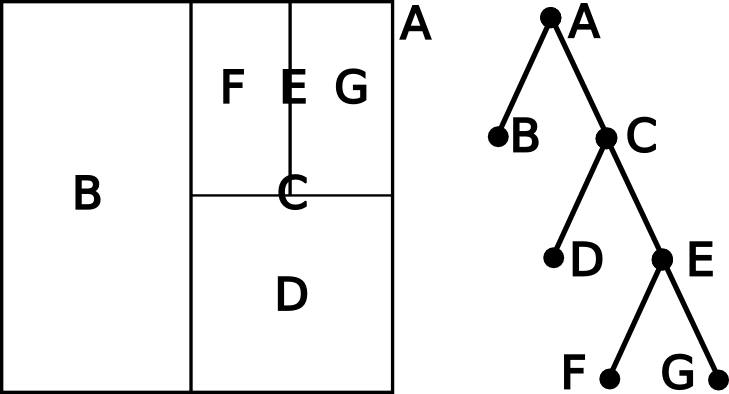
\includegraphics[width=0.5\textwidth]{fig/ex_BSP.png}
     \caption{Uma subdivisão feita com BSP e sua representação em árvore.} 
     \label{fig:ex_BSP}
 \end{figure}
 
 
 
 
 
 
 
 
 
 
 
 
 
 
 
 
 
 
 


\section{Decomposição Baseada na Distância/Volume/Centro de Massa}


O Trabalho de \cite{bib:VIDWANS94} apresenta uma técnica de particionamento com balanceamento por divisão e conquista, onde pode ocorrer uma redistribuição das cargas dos processadores. Inicialmente os planos de corte são criados baseados na centroide, utilizando os eixos para orientação do plano de corte, podendo criar os cortes sempre em um dos eixos ou então alinhando o plano em relação a mais de um eixo. É criado então conjuntos de vértices, arestas e faces para cada subdomínio criado. Cada subdomínio é atribuído a um processador e são balanceados trocando elementos desses conjuntos com seus vizinhos. Figura \ref{fig:vidwans} mostra um exemplo de balanceamento de carga feito pelo método.


 \begin{figure}[htbp]
     \centering
     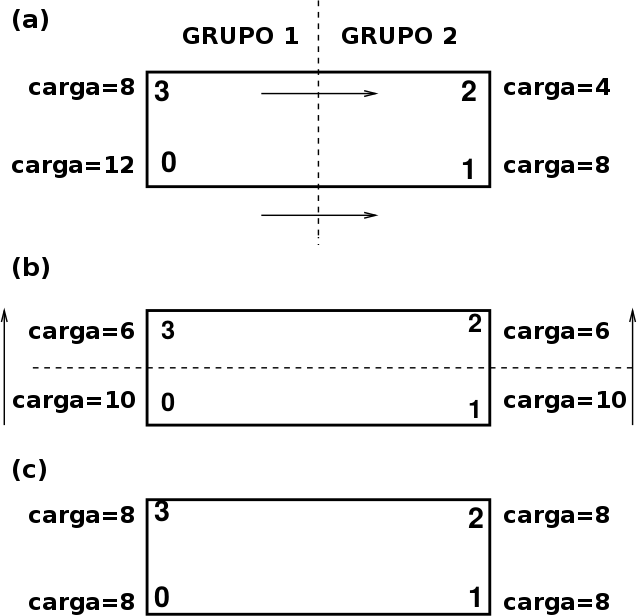
\includegraphics[width=0.5\textwidth]{fig/vidwans.png}
     \caption{Exemplo do método de divisão e conquistar de \cite{bib:VIDWANS94} para equilibrar a carga entre quatro processadores. (a) distribuição de carga inicial. (b) Distribuição de carga após o passo 1. (c) Distribuição de carga após o passo 2.}
     \label{fig:vidwans}
 \end{figure} 

 
No trabalho de \cite{bib:GAITHER96} traz uma técnica de geração de malha bidimensional por inserção de pontos com decomposição Discreta. Ela é baseada na área dos sub-domínios e na área dos triângulos que estão sendo gerados, não possuindo assim nenhuma estimativa de carga. Inicialmente é gerada uma malha grosseira com os vértices de entrada e depois é realizado um agrupamento dos triângulos, de tal forma que ao final a quantidade de regiões e processadores sejam iguais. As fronteiras das regiões criadas são discretizadas e um algoritmo de Delaunay bidimensional é aplicado. A Figura \ref{fig:gaither} mostra o passo a passo da técnica.

 
 \begin{figure}[htbp]
     \centering
     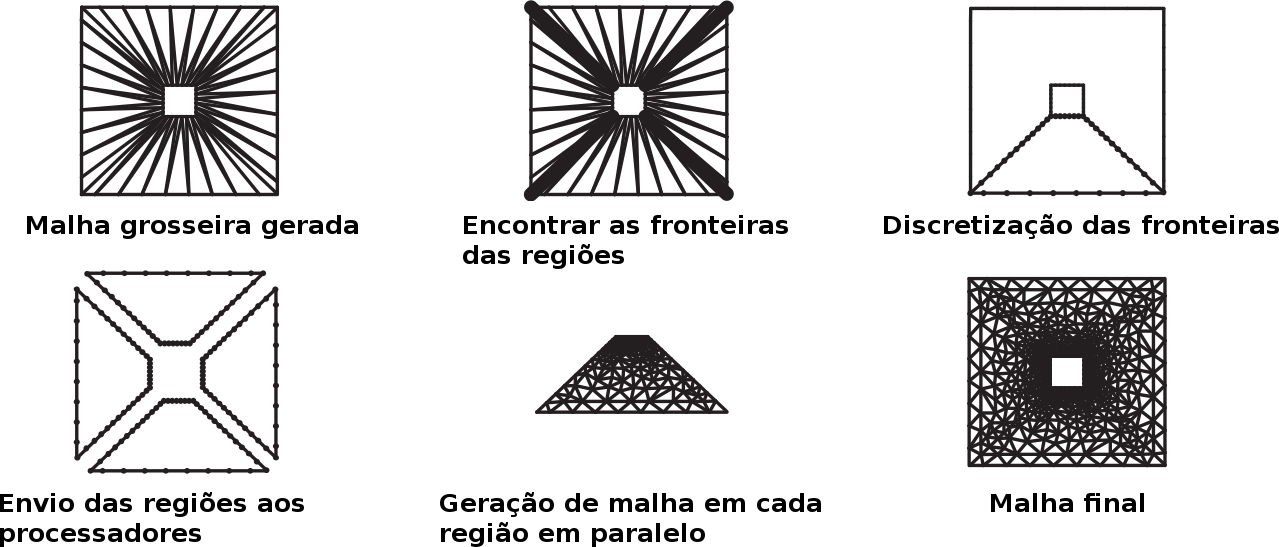
\includegraphics[width=1.0\textwidth]{fig/gaither.png}
     \caption{Passo a passo da técnica de \cite{bib:GAITHER96}.}
     \label{fig:gaither}
 \end{figure} 

 
 Em \cite{bib:WU96}, uma técnica de decomposição Discreta é descrita. O particionamento é feito numa malha inicial grosseira. É identificado os sub-domínios nesta malha grosseira com base na carga (área da região), no tamanho da interface e conectividade entre regiões. Após ter os subdomínios definidos, é feito um refinamento na malha inicial grosseira. Ao final os subdomínios são redefinidos com base na nova malha. A Figura \ref{fig:wu} ilustra o passo a passo da técnica. O trabalho de \cite{bib:BANK05} tem uma metodologia parecida, onde utiliza uma malha grosseira para realizar o particionamento, que é baseado na bisseção. 
 
 \begin{figure}[htbp]
     \centering
     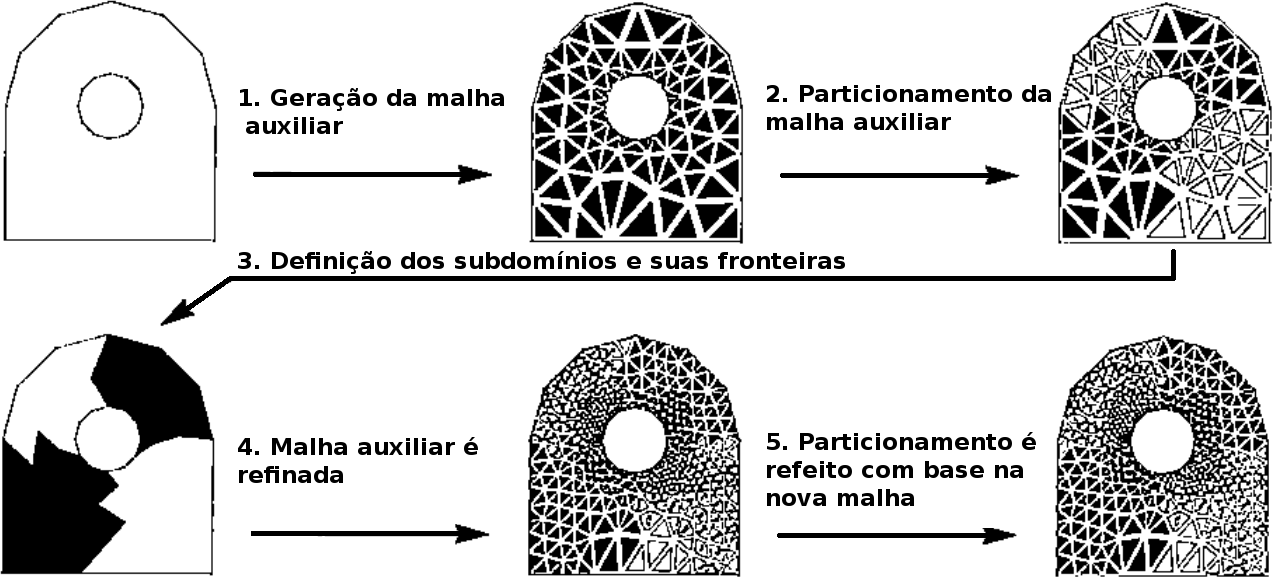
\includegraphics[width=0.8\textwidth]{fig/wu.png}
     \caption{O passo a passo da técnica de \cite{bib:WU96}.}
     \label{fig:wu}
 \end{figure}  

 
 Em \cite{bib:GALTIER96} permite utilizar duas abordagens para decomposição. A primeira é pela decomposição em um mesmo eixo pela distancia entre dos planos de corte. A segunda é pela decomposição recursiva onde os planos de cortes passam pelo momento de inércia. A malha das interfaces são criadas por um grafo de Voronoi, que por sua vez vem de uma triangulação de Delaunay dos vértices iniciais.
 

Em \cite{bib:SAID99} apresenta uma técnica de decomposição Discreta que utiliza uma grade volumétrica para auxiliar na decomposição. A estimativa de carga é realizada pela quantidade de faces presentes numa região. Tanto a malha quanto a grade volumétrica são geradas por Delaunay. As subdivisões são feitas considerando também o volume das regiões. A Figura \ref{fig:said} mostra um exemplo da formação dos subdomínios em


 \begin{figure}[htbp]
     \centering
     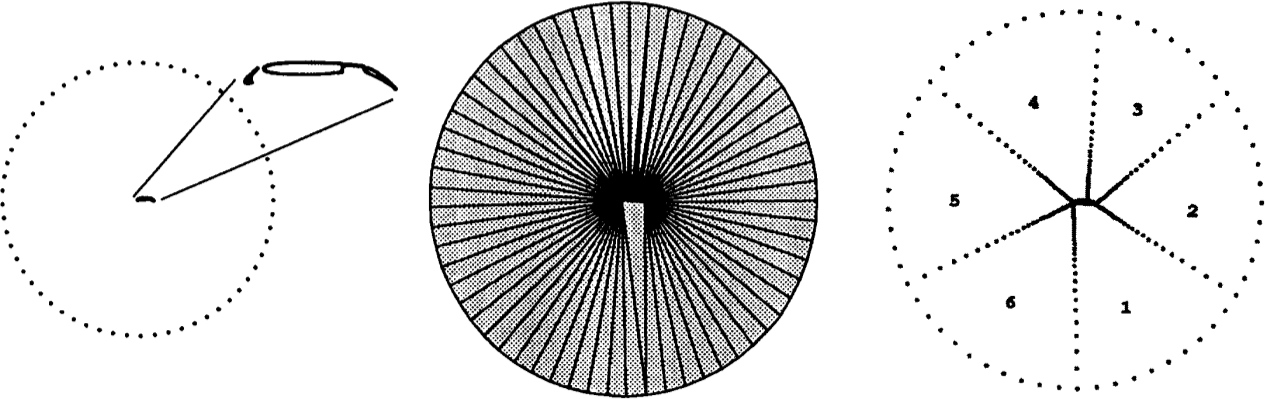
\includegraphics[width=0.9\textwidth]{fig/said.png}
     \caption{Exemplo da formação dos subdomínios em \cite{bib:SAID99}. Fronteira de entrada, grade auxiliar inicial e 6 subdomínios gerados juntamente com as suas discretizações respectivamente.}
     \label{fig:said}
 \end{figure} 


Em \cite{bib:Ivanov06}, foi desenvolvido um algoritmo \textit{a priori} baseado em Delaunay para geração de malhas tetraédricas em que o posicionamento do plano de corte é definido pelo centro de massa e pela matriz de inércia. O plano de corte é um plano perpendicular a um eixo que segue uma das três definições:

\begin{itemize}
  \item Planos criados são equidistantes;

  \item Volume entre os planos são iguais;

  \item Passa pelo centro de massa.
\end{itemize}

A escolha do critério utilizado para criar os subdomínios depende da geometria da entrada. Assim, dependendo da entrada, um critério pode ser melhor que outro, mas isso depende do conhecimento do usuário. Na Figura~\ref{fig:ivanov06}, as três formas de decomposição são apresentadas.

Após ter o plano de corte definido, é feita uma suavização da seção de corte e a sua triangulação para, posteriormente, serem geradas as malhas nos subdomínios. Um problema bem visível nesse método é que para se ter um bom plano de corte é preciso ter um modelo com uma geometria bem comportada, sem forma côncava, alongada ou afinada. Nesse trabalho a quantidade de subdomínios gerados é maior que a de processos para tentar melhorar o balanceamento dinâmico, uma vez que não se tem uma boa precisão na estimativa da carga.

 \begin{figure}[htbp]
     \centering
     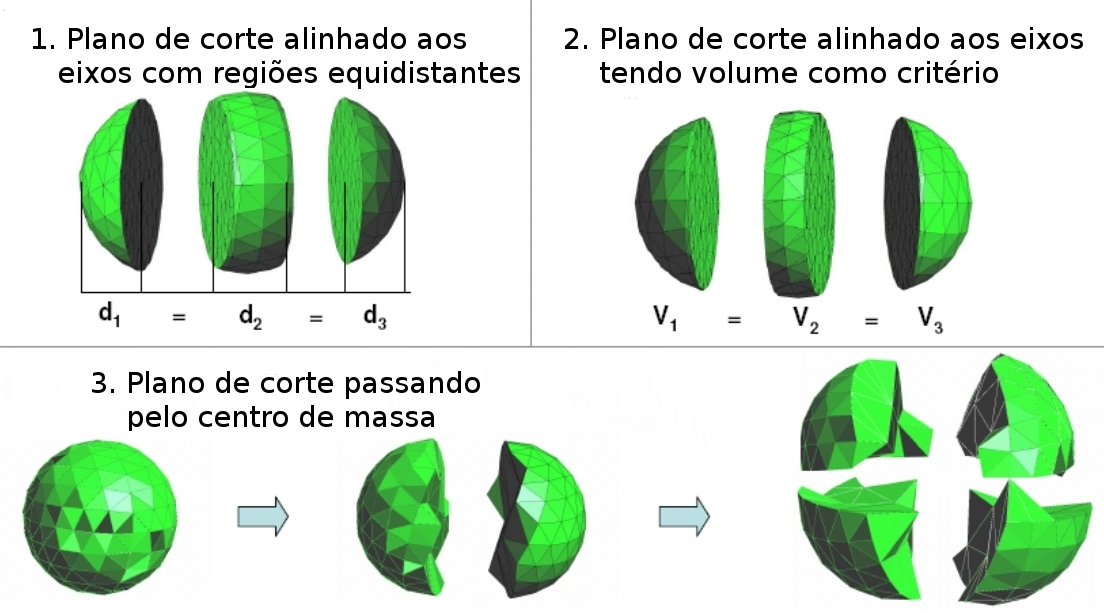
\includegraphics[width=0.9\textwidth]{fig/ivanov06.jpg}
     \caption{As três formas de particionar. 1 - planos equidistantes. 2 - volume dos subdomínios iguais. 3 - centro de massa \cite{bib:Ivanov06}.}
     \label{fig:ivanov06}
 \end{figure}

Uma solução parecida é a apresentada em \cite{bib:Lammer00}, em que o plano de corte é traçado da mesma maneira, porém em duas dimensões, ou seja, um eixo de corte. Este eixo é usado para dividir o domínio recursivamente. A partir do eixo, uma aresta é formada, e os valores nos seus pontos extremos são interpolados dos valores dados como entrada. Quando o número de subdomínios for igual ao número de processadores, uma malha de Delaunay é gerada em cada interior concorrentemente. Essa técnica não apresenta uma boa escalabilidade nos seus resultados.


\cite{bib:JURCZYK07} apresenta uma técnica de decomposição \textit{a priori} onde o plano de corte é criado segundo um série de requisitos. Entre os requisitos estão que o volume das regiões geradas devem ser aproximadamente a mesmo, o plano de corte deve ser mínimo, os seja, poucos elementos pertencem ao separador e o ângulo de junção com a fronteira de entrada não deve formar um ângulo agudo. O balanceamento desta técnica é feito pela quantidade de faces na superfície. A Figura \ref{fig:jurczyk} mostra o processo de decomposição.

 
 \begin{figure}[htbp]
     \centering
     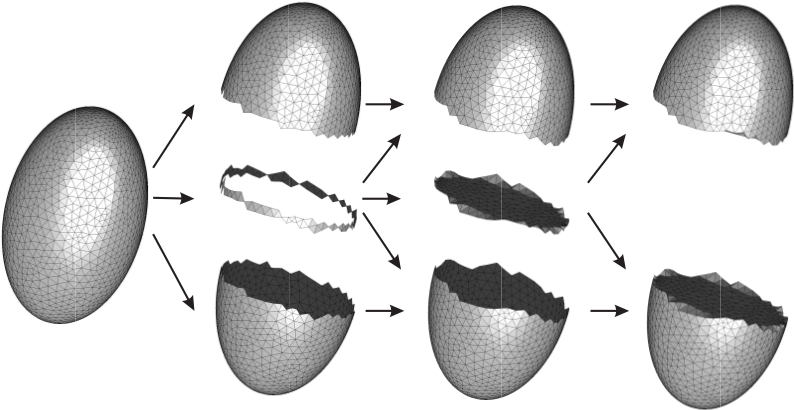
\includegraphics[width=0.7\textwidth]{fig/jurczyk.png}
     \caption{Exemplo do processo de decomposição em \cite{bib:JURCZYK07}.}
     \label{fig:jurczyk}
 \end{figure} 


Em \cite{bib:ANDRA08}, é utilizado o centro de massa e o momento de inercia para encontrar os planos de corte do domínio. As interfaces são geradas \textit{a priori} por Delaunay bidimensional e convertidas depois para tridimensional. A Figura \ref{fig:andra} mostra um exemplo de particionamento feito pela técnica.

 \begin{figure}[htbp]
     \centering
     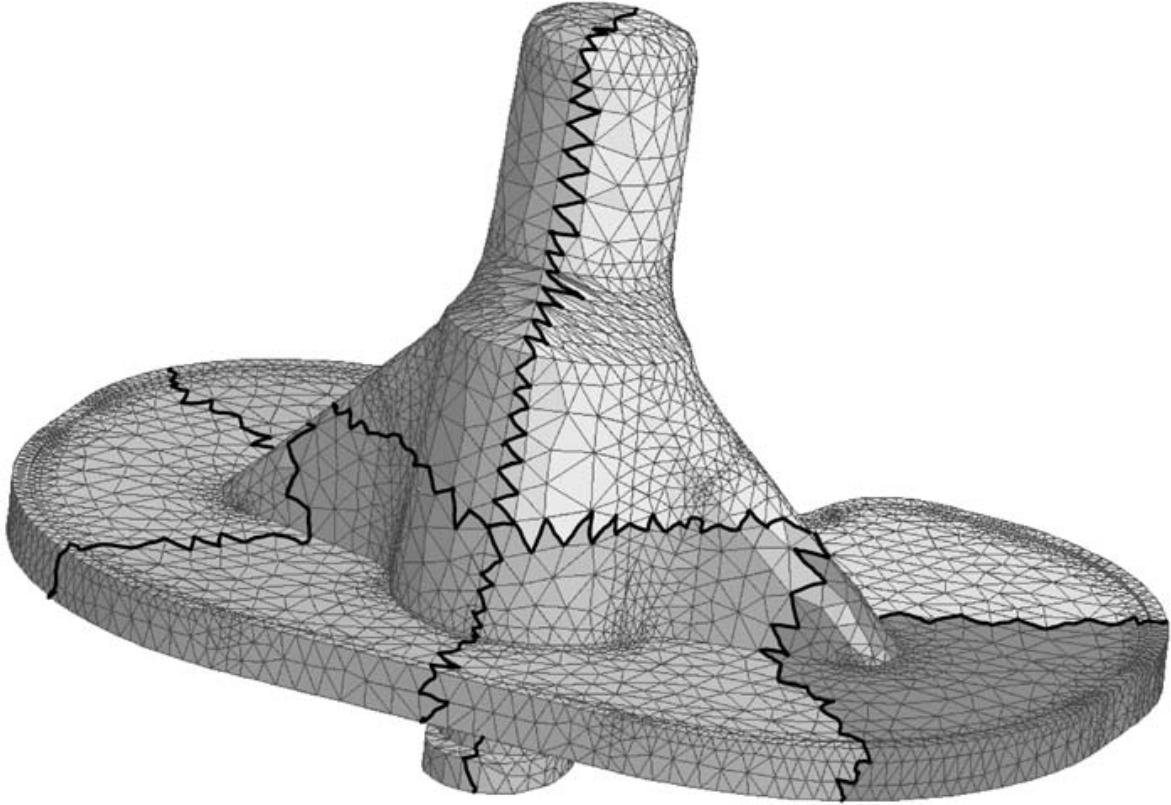
\includegraphics[width=0.6\textwidth]{fig/andra.png}
     \caption{Exemplo de uma decomposição feita por \cite{bib:ANDRA08} para 8 subdomínios.}
     \label{fig:andra}
 \end{figure}


Em \cite{bib:Pirzadeh09}, é descrita uma técnica baseada em Avanço de Fronteiras e Avanço de Camadas com decomposição contínua \textit{a priori}.

Inicialmente, é gerada uma malha de superfície nos pontos dados como entrada. Logo em seguida, é feita uma estimativa de carga nos subdomínios utilizando uma \textit{octree} que usa a informação da quantidade de faces para subdividir o domínio. Se necessário, serão criados planos de partições que dividem o domínio em regiões com cargas aproximadamente iguais. As posições destes planos são definidas através do centro de densidade da malha. Esse centro indica onde a massa efetiva do sistema está concentrada.

Em seguida, são identificadas as faces que interceptam o plano de partição e uma malha parcial é gerada na região do plano de corte. Depois disso, para cada lado da partição são agrupadas as faces dos novos subdomínios. Esse processo é repetido até que um número máximo de subdivisões tenha ocorrido. Ao final da execução, tem que ser realizada uma junção de todas as submalhas. A Figura~\ref{fig:pirzadeh09} ilustra os principais passos dessa técnica para o caso bidimensional. Esta técnica gera malha por Avanço de Fronteira e é uma mistura de \textit{a priori} com \textit{a posteriori}, pois avança uma camada de elementos na interface para depois criar os subdomínios.

 \begin{figure}[htbp]
     \centering
     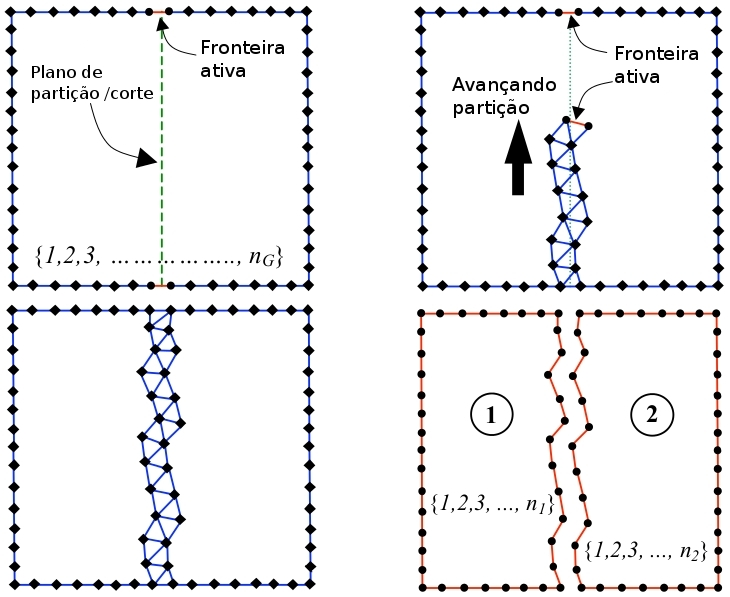
\includegraphics[width=0.8\textwidth]{fig/pirzadeh09.jpg}
     \caption{Os principais passos da técnica de \cite{bib:Pirzadeh09} para gerar os segmentos de interface.}
     \label{fig:pirzadeh09}
 \end{figure}
 
Como vantagens pode-se citar que a utilização de avanço de camadas entre as partições faz com que a malha gerada seja praticamente idêntica a uma malha gerada sequencialmente, ou seja, não são gerados padrões entre as partições do domínio. Outra vantagem é que não é necessário nenhum pré-processamento custoso para definir ou construir as partições. Além disso, a construção da \textit{octree} para estimar a carga é automática e de baixo custo.

Uma das desvantagens desse método é que nem sempre é fácil gerar as malhas nas partições, especialmente em três dimensões. Além disso, a qualidade dessas malhas pode ser ruim, prejudicando assim a qualidade da malha gerada no modelo todo. Basear a quantidade de subdivisões num número máximo não é uma boa métrica para controlar a geração dos subdomínios quando não se tem uma boa estimativa de carga, isso pode gerar subdomínios em excesso, aumentando a comunicação entre os processos. 
 
 
Em \cite{bib:CHEN12} é apresentado uma técnica \textit{a priori} onde o plano de partição é posicionado usando o centro gravitacional para posicionar o plano de corte, juntamente como eixo de inercia para dar a normal do plano. Após isto é encontrado as arestas que fazem interseção com o plano de corte, eliminando aquelas que tenham vértices com vizinhança menor que dois, nas arestas restantes é realizado uma suavização (Figura \ref{fig:chen}). A interface é gerada por Delaunay nas arestas da fronteira encontrada. Apesar do esforço para a criação de uma boa interface, esta técnica não possui um estimativa de carga clara para os subdomínios, tentando compensar o balanceamento de carga fazendo \textit{over-decomposition} (criação de mais subdomínios que processadores disponíveis). Um trabalho parecido é \cite{bib:ZHENG09}, onde os planos de cortes devem ser os menores possíveis e que gerem subdomínios de tamanhos praticamente iguais. O posicionamento do corte no principal eixo de inércia.


 \begin{figure}[htbp]
     \centering
     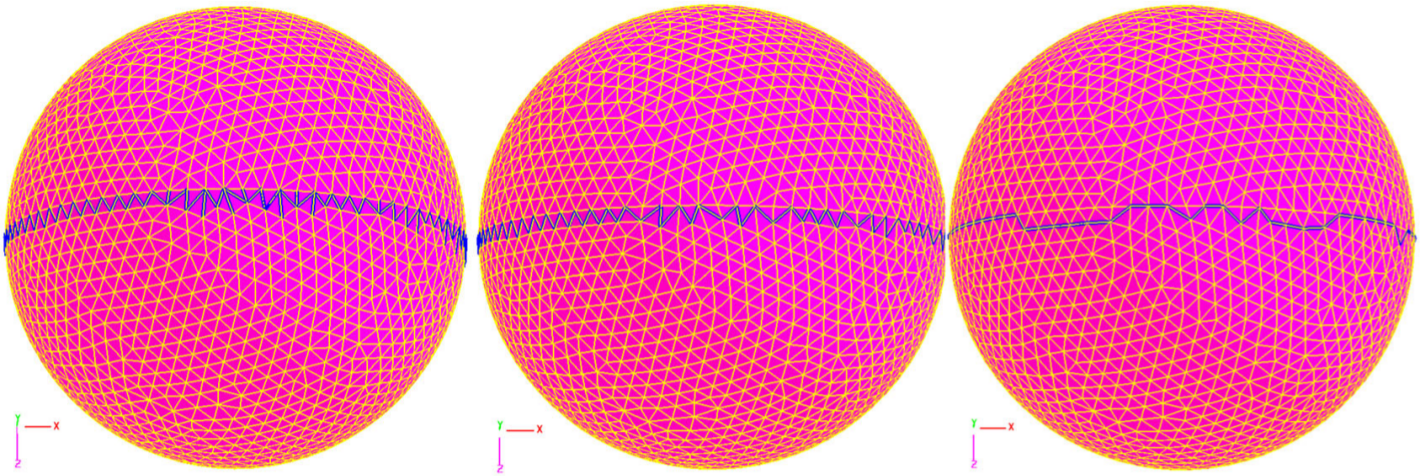
\includegraphics[width=1.0\textwidth]{fig/chen.png}
     \caption{Da esquerda para direita: todas as arestas que sofrem interseção, a fronteira inicial, e a fronteira suavizada. Em \cite{bib:CHEN12}.}
     \label{fig:chen}
 \end{figure}
 
 
\section{Decomposição Baseada em Grafos/Estruturas de Dados tipo Árvore} \label{sec:decomposição_est_dados}


Alguns trabalhos como o de \cite{bib:BARNARD94} utilizam grafos para encontrar o corte no domínio. O corte é baseado num grafo criado com as arestas, maximizando a quantidade de vértices nos conjuntos e minimizando a quantidade de arestas cortadas pelo corte. A criação do grafo para o particionamento é ilustrada na Figura \ref{fig:barnard}. No trabalho de \cite{bib:SIMON91} além desta forma de particionamento, é mostrada também particionamentos feitos pela bisseção e pelo particionamento recursivo da bisseção espectral (autovetores da matriz Laplaciana de um grafo).


\begin{figure}[htbp]
  \centering
  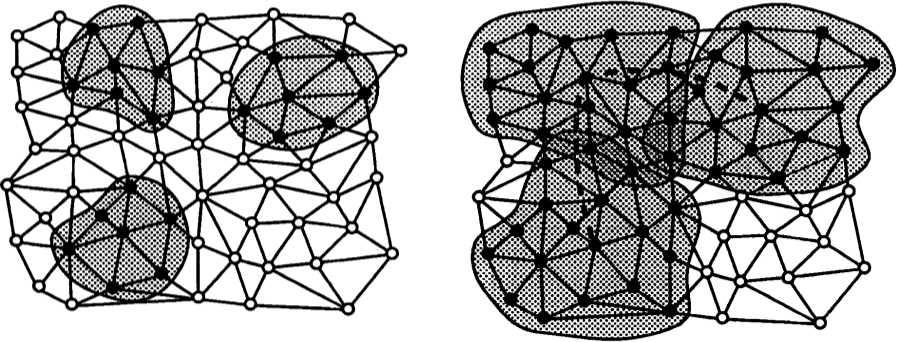
\includegraphics[width=0.8\textwidth]{fig/barnard.png}
   \caption{ Fluxograma da triangulação em paralelo \cite{bib:BARNARD94}.}
  \label{fig:barnard}
\end{figure}


Em \cite{bib:NIKISHKOV99}, um grafo é construído para fazer a estimativa de carga e para realizar o particionamento. O critério de subdivisão é a quantidade de elementos internos a cada subdomínio. A Figura \ref{fig:nikishkov} mostra um exemplo de particionamento para esta técnica.

\begin{figure}[htbp]
  \centering
  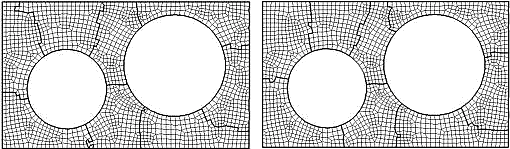
\includegraphics[width=0.8\textwidth]{fig/nikishkov.png}
   \caption{Oito subdomínios criados com quantidades iguais de elementos e do lado direito a otimização das partições em \cite{bib:NIKISHKOV99}. }
  \label{fig:nikishkov}
\end{figure}


Em \cite{bib:deCougny99}, a entrada do algoritmo é o contorno de um objeto. Cada processador fica com parte de uma \textit{octree} distribuída, que define planos de corte do domínio. A malha das células internas é gerada concorrentemente com \textit{templates}. A região entre o contorno e as células internas é preenchida por uma técnica de Avanço de Fronteira, onde são gerados os elementos internos a uma região delimitada pelos planos de corte. Por último é feita a conexão das malhas dos dois lados de cada plano e de suas intersecções. Essa técnica gera muitas partições, já que a cada subdivisão oito novos subdomínios são criados, e, por usar \textit{templates}, esta técnica pode gerar uma quantidade excessiva de elementos, além de possivelmente gerar elementos de qualidade ruim nas regiões próximas ao contorno.

Na técnica de \cite{bib:Lohner01}, é gerada uma \textit{octree} grosseira com relação ao contorno dado como entrada. Após essa geração, as células que contêm a parte da fronteira que gerará os menores elementos são identificadas. Assim, partes da malha, correspondentes a cada célula, são geradas simultaneamente por avanço de fronteira, de maneira que cada parte da malha gerada não possa cruzar as extremidades da célula que a contém. Cada octante sofre então um pequeno deslocamento na diagonal com o intuito de gerar mais elementos. Esse deslocamento elimina quase todas as faces entre duas ou mais células e diminui o tamanho da fronteira para o próximo passo. Desse modo a nova fronteira é encontrada e uma nova \textit{octree} é construída para ela, e o procedimento é repetido, até que não seja mais possível gerar malha. Na Figura \ref{fig:lohner}, são mostrados os passos do algoritmo e os deslocamentos que são realizados.


    \begin{figure}[!ht]
    \centering
    \subfloat[\textit{Octree} gerada para uma borda e passos do algoritmo (representação 2D, ou seja, uma \textit{quadtree}).]
    {\label{fig:lohner1}
     \begin{minipage}[c]{0.45\textwidth}{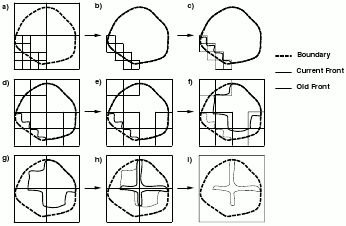
\includegraphics[width=\textwidth]{fig/lohner1.png}}\end{minipage}
    }
    \qquad
    \subfloat[Deslocamento da \textit{quadtree} para gerar mais malha (a linha escura é a fronteira).]
    {\label{fig:lohner2}
     \begin{minipage}[c]{0.45\textwidth}{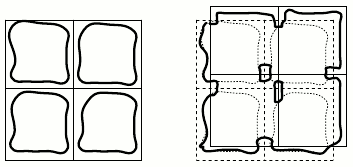
\includegraphics[width=\textwidth]{fig/lohner2.png}}\end{minipage}
    }    
    \caption{Técnica de \cite{bib:Lohner01}.}
    \label{fig:lohner}
    \end{figure}

O deslocamento de cada octante é feito seguindo-se sempre o mesmo processo, e isso pode não ser o ideal para certos tipos de modelos, onde maneiras distintas de deslocamento poderiam ser mais eficientes (deslocamentos na diagonal, na direção dos eixos principais, entre outros).

No trabalho de \cite{bib:LOHNER14} traz algumas técnicas recentes na área de geração de malhas em paralelo. A principal novidade é a utilização da própria estrutura da árvore de decomposição para unir as interfaces dos subdomínios. A utilização da árvore de decomposição já torna a paralelização mais natural e simples (Figura \ref{fig:lohner14}).


 \begin{figure}[htbp]
     \centering
     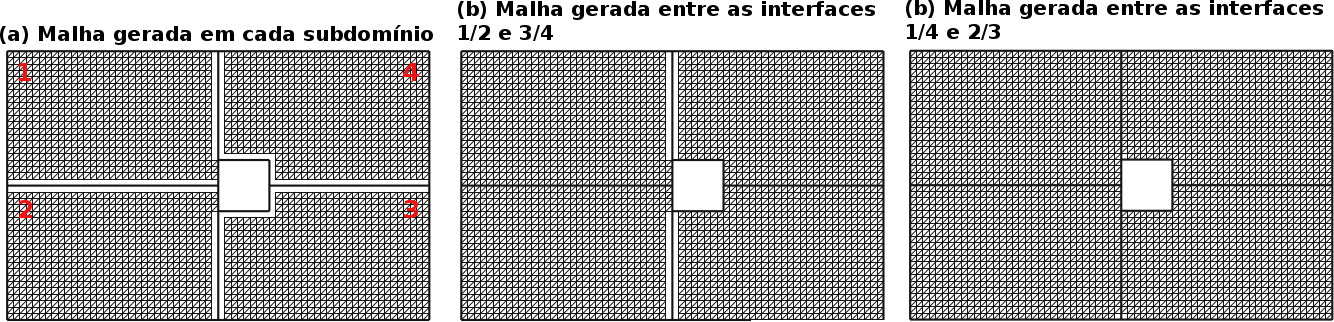
\includegraphics[width=1.0\textwidth]{fig/lohner14.png}
     \caption{Junção das malhas dos subdomínios em \cite{bib:LOHNER14}.}
     \label{fig:lohner14}
 \end{figure}
 

Em \cite{bib:Larwood03}, é apresentada uma técnica de decomposição de domínio que tem como entrada uma triangulação de borda. Para saber quais subdomínios devem ser divididos, a técnica usa um critério baseado na quantidade de faces por subdomínio. A decomposição é feita recursivamente usando uma \textit{octree} caso seja tridimensional ou uma \textit{quadtree} caso seja bidimensional, verificando sempre se o número de faces de um subdomínio é menor do que o limite estipulado, e, enquanto a verificação for falsa, a decomposição ocorre. A quantidade máxima de subdivisões está limitada por uma constante maior que o número de processadores disponíveis. Isso evita a criação excessiva de partições e permite que um processador possa receber mais de uma tarefa ao longo da execução. As interfaces dos subdomínios são geradas \textit{a priori} por Delaunay. A qualidade da malha não é garantida neste trabalho, são apresentados apenas resultados de balanceamento de carga entre os processadores que é garantido pela \
textit{over-decomposition}.

 \begin{figure}[htbp]
     \centering
     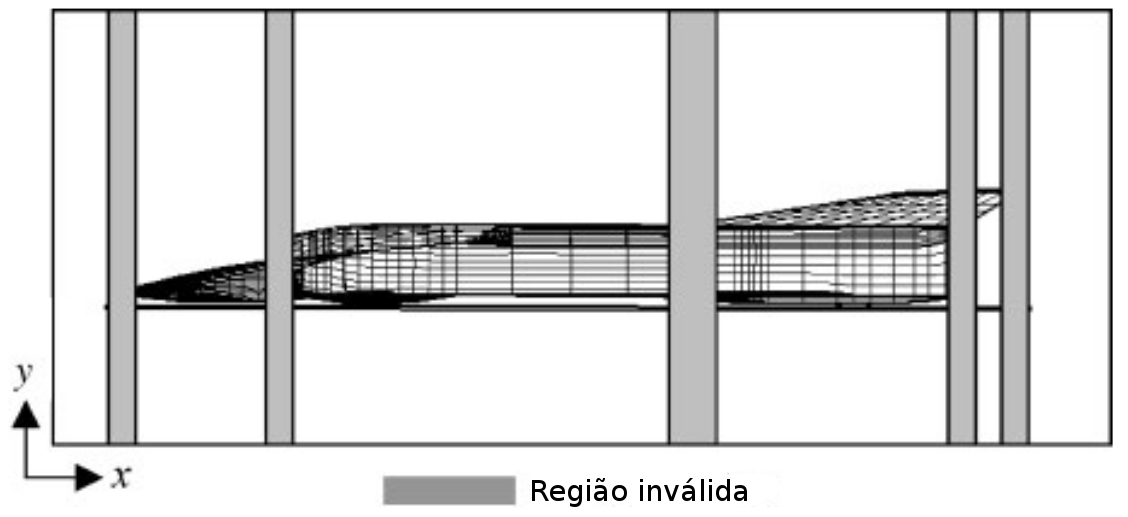
\includegraphics[width=0.8\textwidth]{fig/larwood03.jpg}
     \caption{Regiões de corte inválidas em cinza \cite{bib:Larwood03}.}
     \label{fig:larwood03}
 \end{figure}
 
Para evitar a criação de elementos ruins, é feita uma verificação no corte baseada no ângulo do vetor normal do plano de corte com a normal dos triângulos, de forma que o plano de corte não possa passar por triângulos com ângulo menor do que uma tolerância. Caso essa verificação falhe, a \textit{octree} (\textit{quadtree}, em 2D) sofre um deslocamento em um dos eixos. A Figura~\ref{fig:larwood03} mostra um exemplo onde alguns planos de corte falham nos testes. 

No trabalho de \cite{bib:CHARMPIS05} trabalha com malhas de elementos finitos e é feita uma representação da entrada  como um grafo e em seguida é utilizado um particionador de grafos (SCGEN) que procura dividir os pesos do pesos dos nós e arestas do grafo de acordo com a quantidade de processadores disponíveis. A imagem \ref{fig:dimos} mostra uma malha de elementos finitos e a sua partição como grafo.


\begin{figure}[htbp]
  \centering
  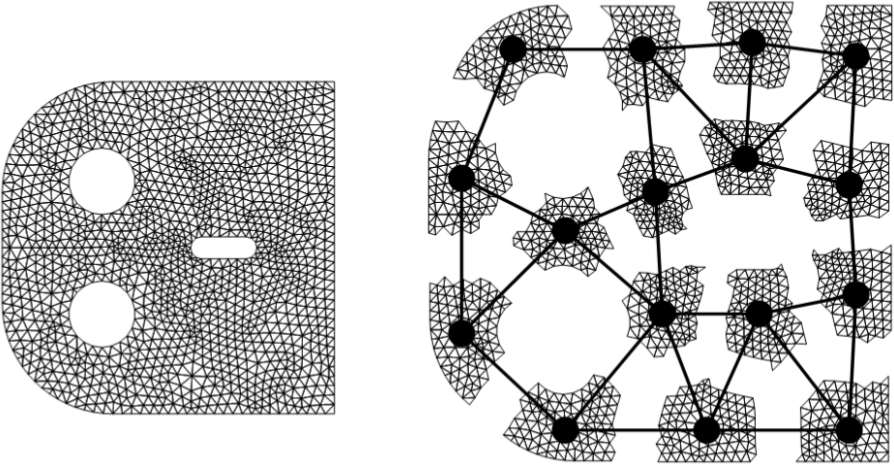
\includegraphics[width=0.6\textwidth]{fig/dimos.png}
   \caption{Malha de elementos finitos (esquerda) e a partição da malha com sua representação em grafo (à direita) em \cite{bib:CHARMPIS05}. }
  \label{fig:dimos}
\end{figure}


Em \cite{bib:Leonidas06}, é apresentada uma técnica bidimensional que utiliza a triangulação de Delaunay por divisão e conquista para um conjunto de pontos dados como entrada. Primeiramente, é feita uma triangulação utilizando apenas os pontos da borda, que é utilizada para a geração de um grafo ponderado, onde o peso de uma aresta é igual ao raio da circunferência circunscrita do triângulo que a contém. Em seguida é feita uma contração desse grafo, onde os vértices do grafo representam a área a ser triangularizada (futuros subdomínios), e as arestas representam a conexão entre essas áreas.
 
Através do grafo formado, os planos de corte são posicionados e os subdomínios formados. A Figura~\ref{fig:leonidas06} mostra o resultado da decomposições para quantidades diferentes de subdomínios. Esse processo de subdivisão ocorre até que a quantidade de subdomínios criados seja suficientemente grande. Isso acontece para tentar melhorar o balanceamento de carga. Após isso, a geração da malha interna poderá ser realizada. A desvantagem dessa técnica é a ausência de uma estimativa de carga eficiente, precisando gerar vários subdomínios para melhorar o balanceamento de carga.

 \begin{figure}[htbp]
     \centering
     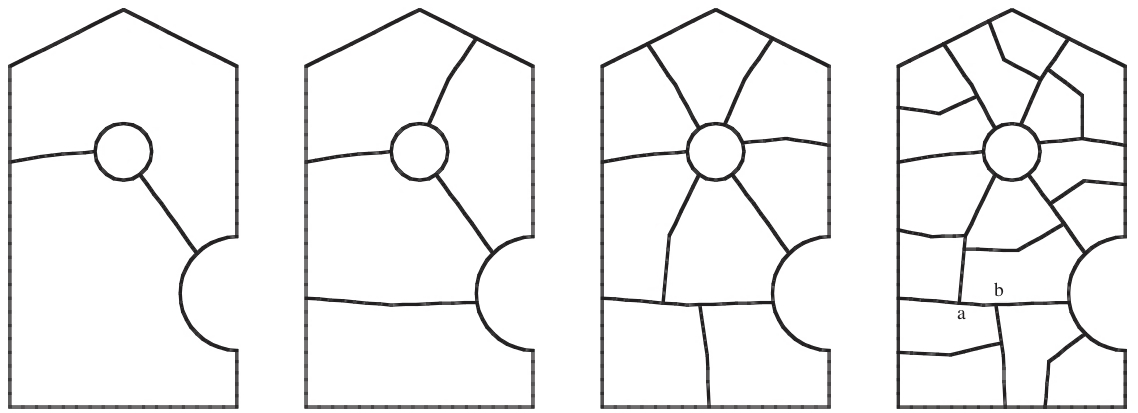
\includegraphics[width=0.7\textwidth]{fig/leonidas06.jpg}
     \caption{Construção do grafo de particionamento de \cite{bib:Leonidas06}.}
     \label{fig:leonidas06}
 \end{figure} 
 

Em \cite{bib:Ito07} o particionador de malhas METIS também é utilizado. Uma malha tetraédrica grosseira é gerada inicialmente com base nas faces da superfície. O particionador de grafos METIS é utilizado para subdividir o domínio tendo como base a malha grosseira gerada. A Figura \ref{fig:ito} mostra para uma esfera o processo de particionamento.


\begin{figure}[htbp]
  \centering
  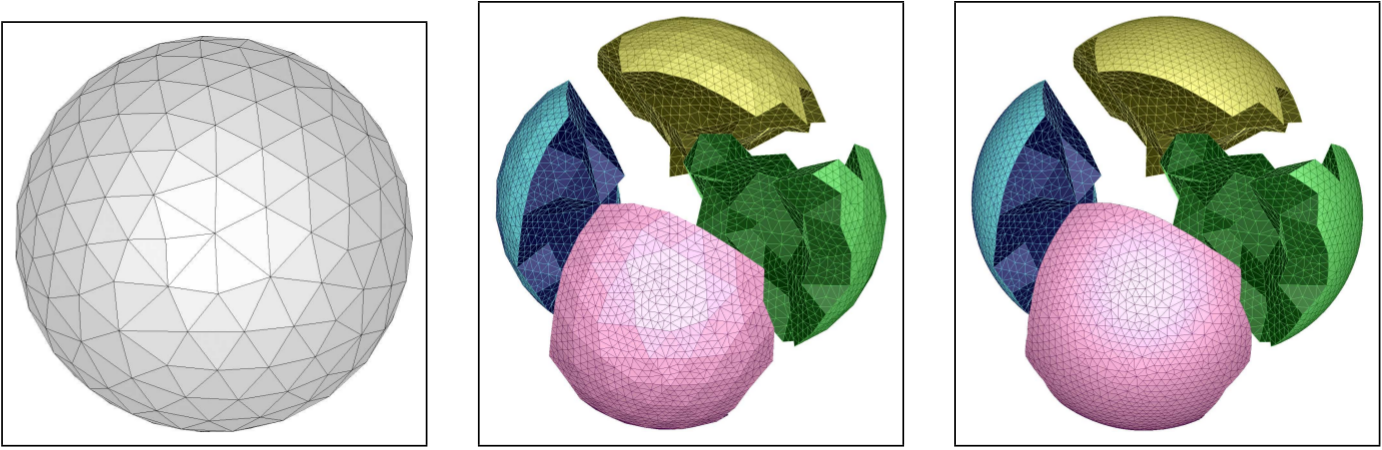
\includegraphics[width=0.8\textwidth]{fig/ito.png}
   \caption{Malha tetraédrica inicial, malha de superfície refinada nos subdomínios e melhorias nas faces de superfície no trabalho de \cite{bib:Ito07}.}
  \label{fig:ito}
\end{figure}

Outro trabalho que também utiliza grafos é o de \cite{bib:PANITANARAK11}, que descreve uma técnica de decomposição Discreta que utiliza o programa de partição de grafos METIS (\cite{bib:Karypis98}). Primeiramente é construída uma malha grosseira com a restrição dos ângulos formados com a fronteira sejam maiores que 30º. Com a malha devidamente criada, é feita a sua conversão para um grafo, onde cada triângulo é representado como um nó e cada aresta como a vizinhança dos triângulos. O particionamento é feito neste grafo de acordo com a quantidade de subdomínios desejado. A Figura \ref{fig:panitanarak} mostra um exemplo de particionamento feito utilizando esta técnica.


\begin{figure}[htbp]
  \centering
  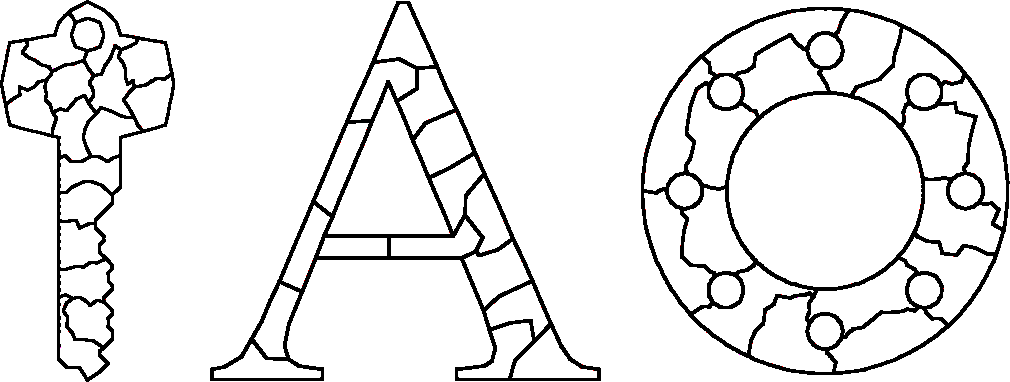
\includegraphics[width=0.6\textwidth]{fig/panitanarak.png}
   \caption{Decomposição feita pela técnica de \cite{bib:PANITANARAK11}.}
  \label{fig:panitanarak}
\end{figure}


Em \cite{bib:Lo12}, uma técnica bidimensional para uma triangulação de Delaunay por inserção de pontos é apresentada. Uma \textit{kd-tree} é utilizada para organizar os pontos da entrada em células. Estas células são agrupadas em zonas e distribuídas entre os processadores. A vantagem de usar uma \textit{kd-tree} é que cada célula tem uma quantidade de pontos aproximadamente igual e a busca espacial é facilitada na hora de fazer a inserção de pontos em uma região. A Figura~\ref{fig:lo12_1} mostra a organização de um conjunto de pontos por partição regular e por \textit{kd-tree}.
 
 
 \begin{figure}[htbp]
     \centering
     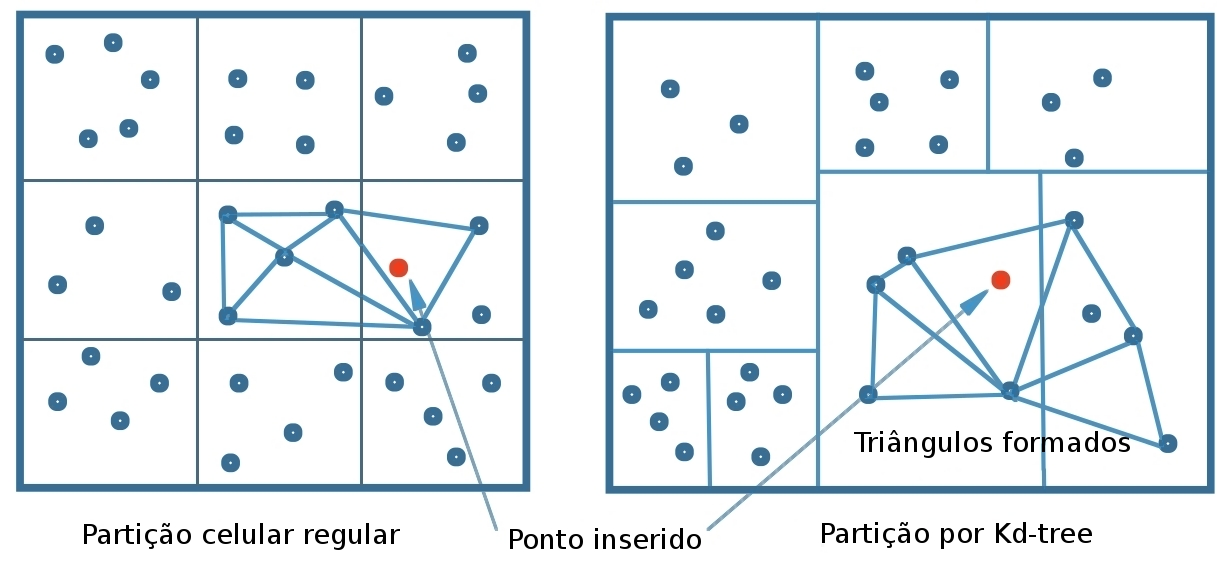
\includegraphics[width=0.8\textwidth]{fig/lo12_1.jpg}
     \caption{Pontos organizados em células. À esquerda por partição regular e à direita por \textit{kd-tree} \cite{bib:Lo12}.}
     \label{fig:lo12_1}
 \end{figure} 

 
A quantidade de subdomínios criados é compatível com a quantidade de processadores disponíveis, ou seja, cada processador terá que ficar responsável por uma zona. A inserção dos pontos em cada zona é feita em paralelo, sendo totalmente independente das outras zonas, e a malha gerada em cada zona também será independente.
 
Os triângulos gerados nas bordas das zonas têm pontos de uma zona vizinha. Isso irá gerar uma camada a mais de triângulos nas zonas, que é necessário para obter uma malha sem buracos entre elas. Ao final, tem de ser feita a junção de todas as malhas geradas em uma só e, para isso, é preciso eliminar as redundâncias (triângulos repetidos entre duas zonas). Essa junção das malhas pode ser um processo complexo em determinados modelos e isso pode prejudicar o desempenho do algoritmo. A Figura~\ref{fig:lo12_2} mostra o fluxograma da triangulação em paralelo.
 
   \begin{figure}[htbp]
     \centering
     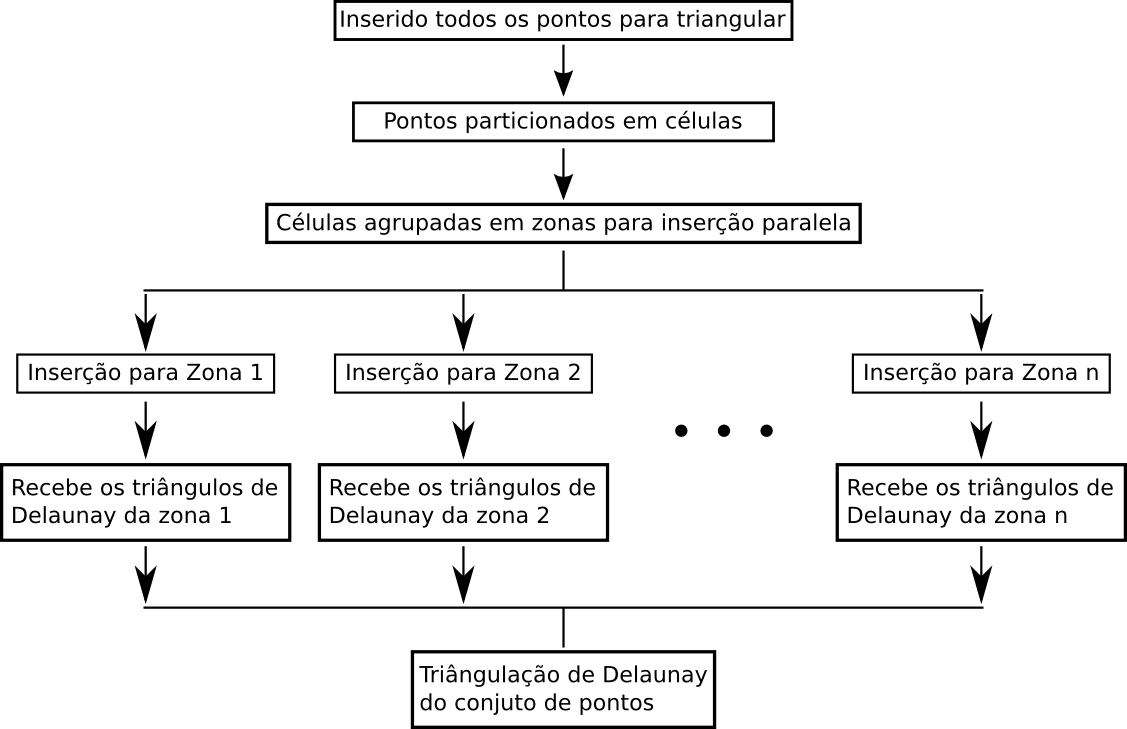
\includegraphics[width=0.8\textwidth]{fig/lo12_2.png}
     \caption{ Fluxograma da triangulação em paralelo \cite{bib:Lo12}.}
     \label{fig:lo12_2}
 \end{figure}

 O trabalho de \cite{bib:MFreitas13} apresenta uma técnica bidimensional que recebe como entrada uma fronteira e utiliza uma \textit{quadtree} para particionar e estimar a carga. As células folhas da \textit{quadtree} de particionamento são divididas entre os processadores disponíveis, onde são geradas as malhas internas. Depois de gerar as malhas nos subdomínios iniciais, a fronteira é atualizada e as células da \textit{quadtree} são deslocadas nos eixos cartesianos a fim de gerar mais malha. Esse processo de deslocamento e geração de malha é feito até que não seja mais possível gerar malha. Um processo mestre fica responsável por finalizar a geração da malha e fazer a melhoria na mesma. Este trabalho é classificado como contínuo \textit{a posteriori}. A Figura~\ref{fig:mfreitas} ilustra o passo de deslocamento da \textit{quadtree} no eixo X.
 
  \begin{figure}[htbp]
     \centering
     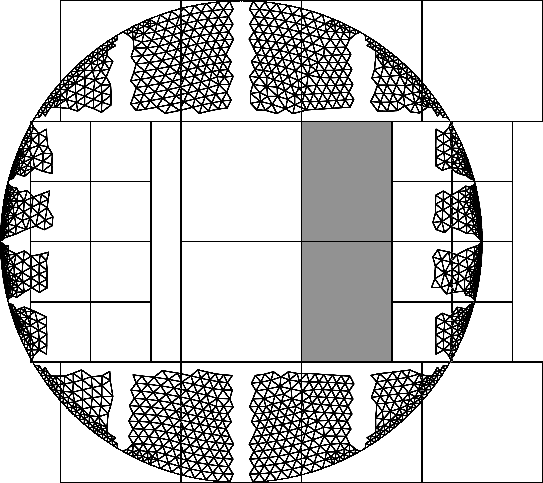
\includegraphics[width=0.4\textwidth]{fig/decomposition_quadtree_shift.png}
     \caption{ Malha gerada, espalhada entre os processos escravos, e as células da \textit{quadtree} de decomposição deslocadas para a direção +X \cite{bib:MFreitas13}.}
     \label{fig:mfreitas}
 \end{figure}
 
 
Em \cite{bib:RepMarkos13}, é apresentada uma evolução da técnica anterior que pode ser tanto bidimensional como tridimensional, por Avanço de Fronteira, com subdivisão baseada em BSP, que recebe como entrada uma superfície de faces triangulares ou uma lista de arestas, para o caso bidimensional. Inicialmente uma \textit{octree} é construída para estimar a carga no domínio de acordo com o tamanho das faces da superfície. As células internas da \textit{octree} têm o tamanho definido de acordo com a maior e a menor face da superfície de entrada. Uma BSP é utilizada para particionar o domínio de tal forma que a quantidade de subdomínios criados seja igual à quantidade de processadores disponíveis.

Após o particionamento, cada subdomínio pertencente a uma folha da árvore BSP gera sua malha por avanço de fronteira até que não seja mais possível avançar (quando chega no plano criado pela BSP), como mostra a Figura \ref{fig:passo_markos1}. Quando os dois filhos de um nó da BSP terminam de gerar a malha nos seus respectivos subdomínios, o nó pai fica encarregado de juntar as duas malhas e, se necessário, terminar a geração da malha no novo subdomínio criado pela junção dos dois filhos, como mostra as Figuras \ref{fig:passo_markos2}, \ref{fig:passo_markos3} e \ref{fig:passo_markos4}.

    \begin{figure}[h]
    \centering
    \subfloat[Malha gerada nas folhas da árvore da BSP.]
    {\label{fig:passo_markos1}
     \begin{minipage}[c]{0.35\textwidth}{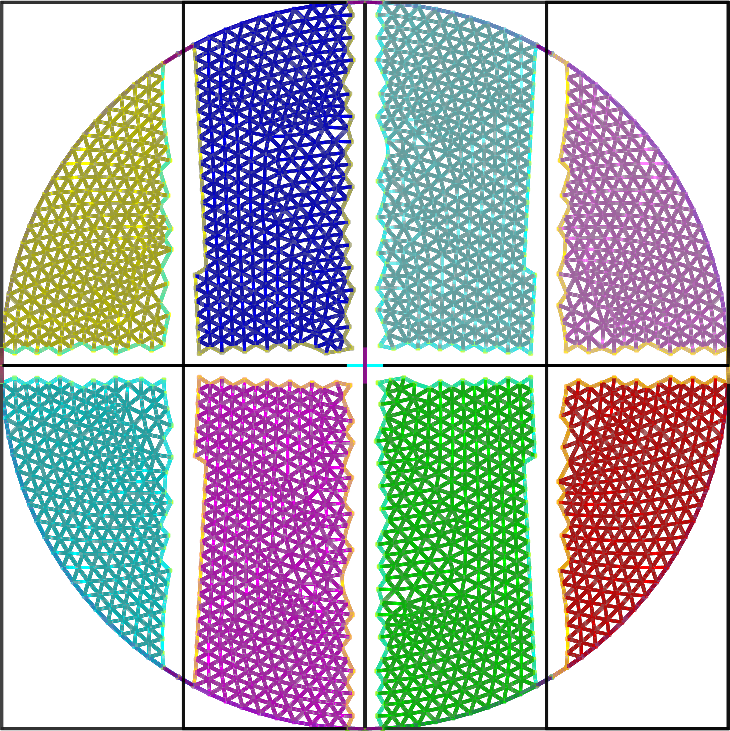
\includegraphics[width=\textwidth]{fig/passo_markos1.png}}\end{minipage}
    }
    \qquad
    \subfloat[Junção e geração da malha no terceiro nível da árvore da BSP.]
    {\label{fig:passo_markos2}
     \begin{minipage}[c]{0.35\textwidth}{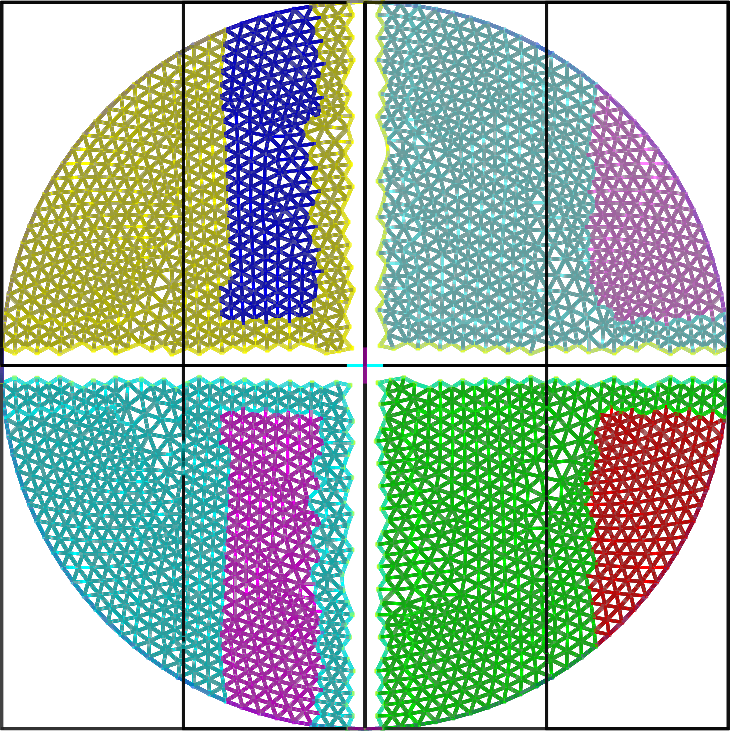
\includegraphics[width=\textwidth]{fig/passo_markos2.png}}\end{minipage}
    }
    
    \subfloat[Junção e geração da malha no segundo nível da árvore da BSP.]
    {\label{fig:passo_markos3}
     \begin{minipage}[c]{0.35\textwidth}{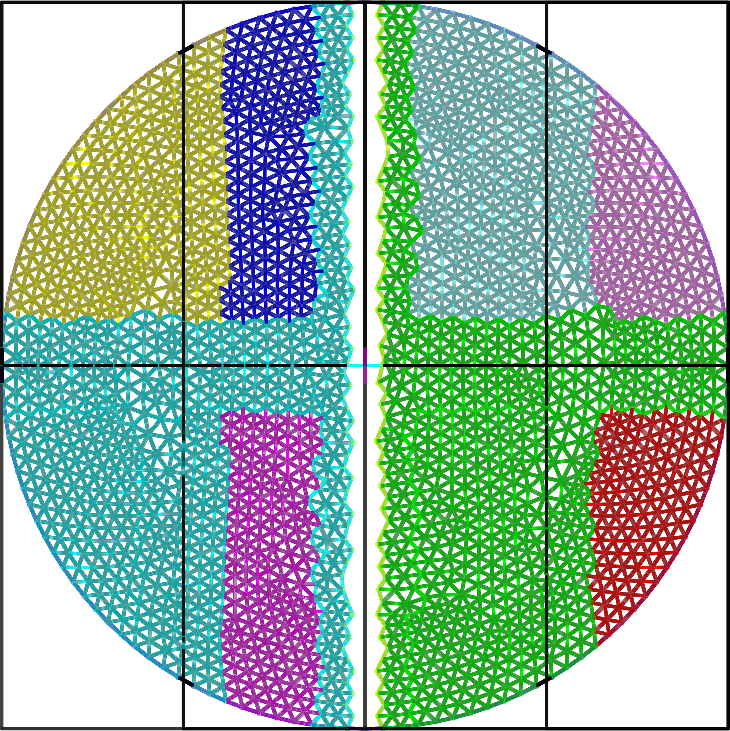
\includegraphics[width=\textwidth]{fig/passo_markos3.png}}\end{minipage}
    }    
    \qquad
    \subfloat[Malha final utilizando particionamento baseado em BSP.]
    {\label{fig:passo_markos4}
     \begin{minipage}[c]{0.35\textwidth}{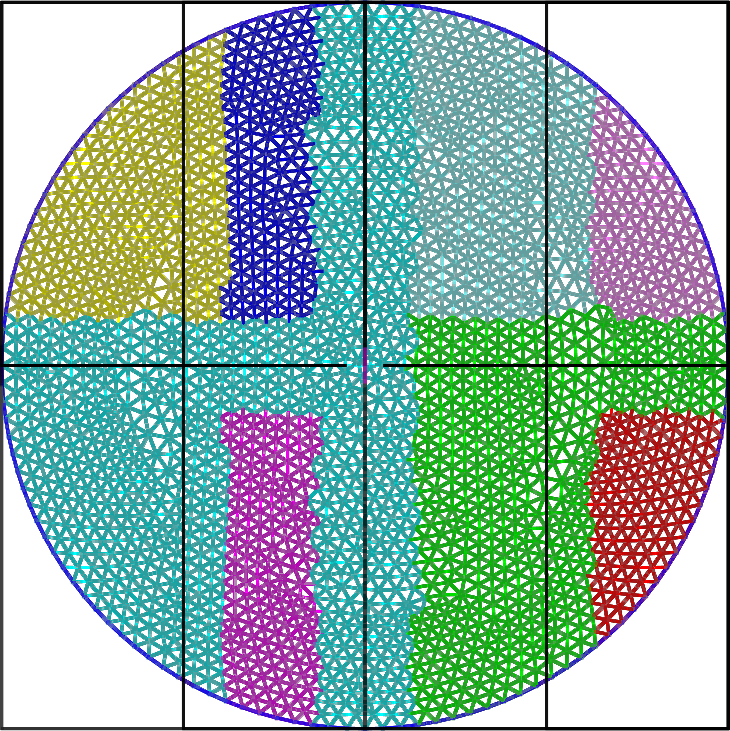
\includegraphics[width=\textwidth]{fig/passo_markos4.png}}\end{minipage}
    }
    \caption{Passos da geração da malha no trabalho de \cite{bib:RepMarkos13}. Cada cor representa a malha gerada por um processador.}
    \label{fig:tecnica Markos 2013}
    \end{figure}

    
A grande vantagem dessa técnica está na utilização da BSP, que acaba permitindo a geração de subdomínios com cargas mais equilibradas e no ganho de velocidade ao se evitar os deslocamentos que aconteciam anteriormente. Por essa abordagem necessitar de uma sincronização e junção da malha em cada nível da BSP, há uma perda na velocidade apesar dessas junções serem feitas em paralelo por processos diferentes.


 \section{Decomposição Baseada em \textit{Bounding Box}}

Um dos primeiros trabalhos em decomposição de domínios foi o de \cite{bib:FARHAT88}, que desenvolveu uma técnica para decomposição de malhas de elementos finitos. Esta técnica subdividia um domínio de acordo com a quantidade de processadores disponíveis, esta técnica utiliza a própria estrutura da malha quadrangular de matriz/grade usando uma estrutura de grade que contém os elementos e realizando o particionamento e a estimativa de carga em cima desta matriz de elementos. A Figura \ref{fig:farhat} mostra um exemplo de decomposição.


 \begin{figure}[htbp]
     \centering
     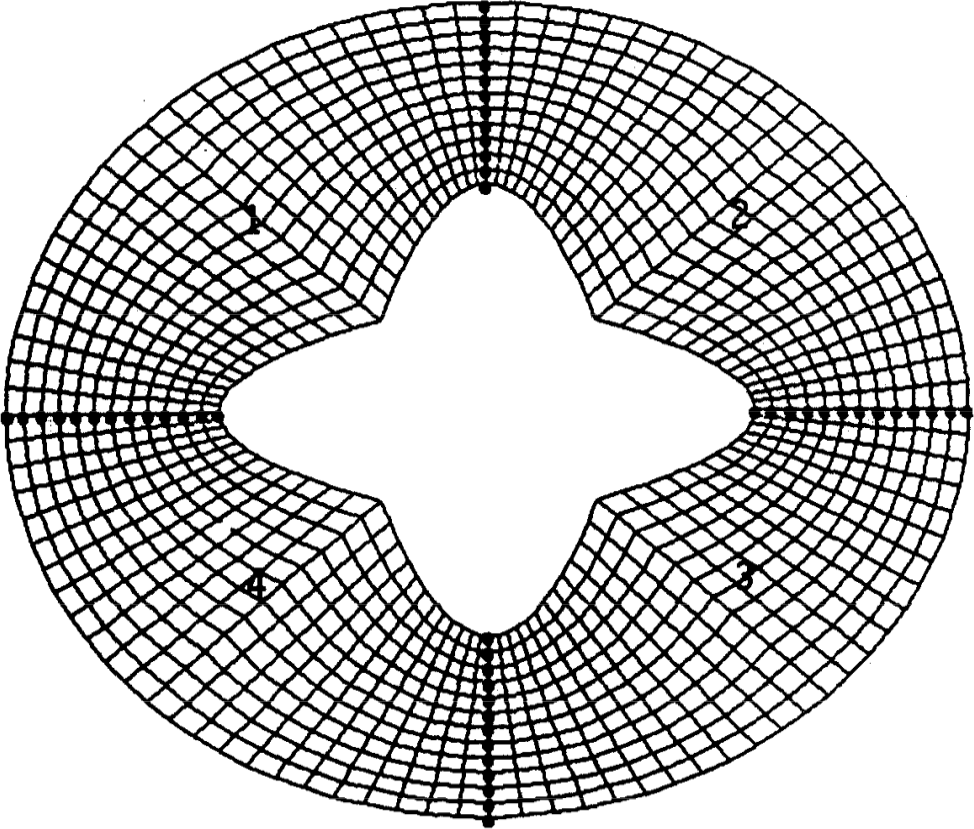
\includegraphics[width=0.4\textwidth]{fig/farhat.png}
     \caption{Decomposição em 4 subdomínios de uma malha multiconectada na técnica de \cite{bib:FARHAT88}.}
     \label{fig:farhat}
 \end{figure}


Em \cite{bib:Glut08}, é apresentada uma técnica para malhas tridimensionais com uma abordagem baseada na decomposição geométrica onde a entrada é uma malha de superfície. Nesse trabalho são descritas duas técnicas baseadas na \textit{bounding box} gerada a partir da entrada.

A seleção do separador do domínio deve garantir um custo de corte baixo, ou seja, encontrar e posicionar o plano de corte não pode ter um custo computacional alto. Além disso, deve garantir um bom balanceamento de carga e minimizar os elementos conectados por múltiplos subdomínios.

A primeira técnica é baseada na malha de superfície. Para o plano de corte ser criado, é preciso a localização do contorno da malha de superfície e do separador. O contorno é então projetado no separador usando uma função 2D de controle espacial baseada no tamanho das arestas (Figura~\ref{fig:glut08_1}).

 \begin{figure}[htbp]
     \centering
     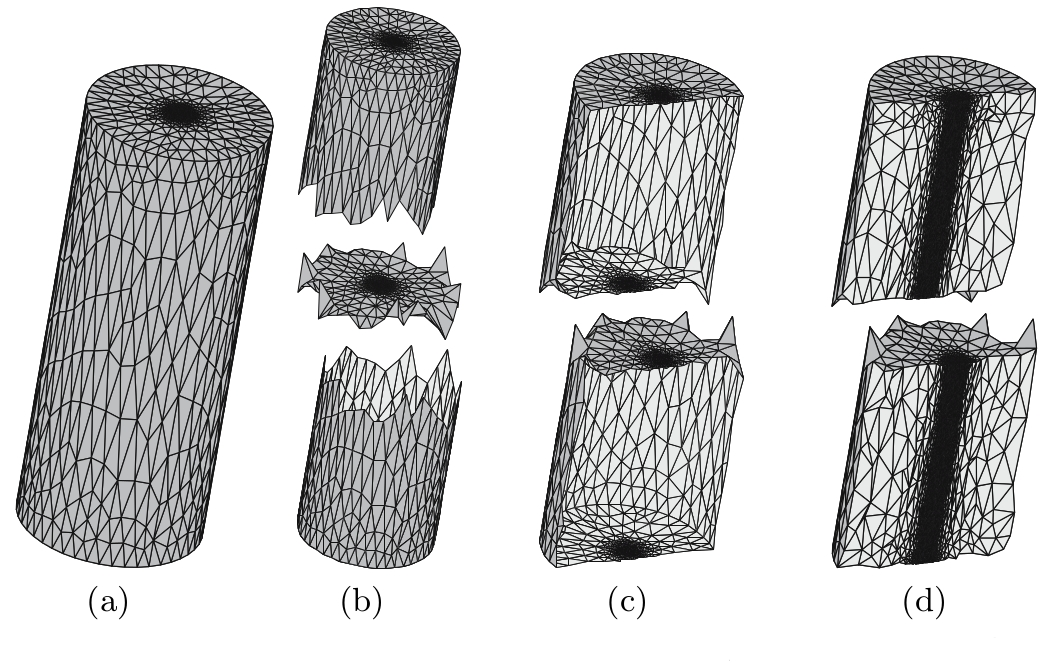
\includegraphics[width=0.8\textwidth]{fig/glut08_1.jpg}
     \caption{Passos da técnica baseada na malha de superfície. (a) malha de superfície; (b) corte; (c) seção transversal; (d) malha final \cite{bib:Glut08}.}
     \label{fig:glut08_1}
 \end{figure}

A segunda técnica se baseia numa malha volumétrica grosseira. Primeiramente, é feita a geração de uma malha 3D grosseira utilizando alguma função de controle espacial. O posicionamento do plano de corte é feito parecido com a técnica anterior, porém utilizando a malha volumétrica como função espacial (Figura~\ref{fig:glut08_2}).

 \begin{figure}[!ht]
     \centering
     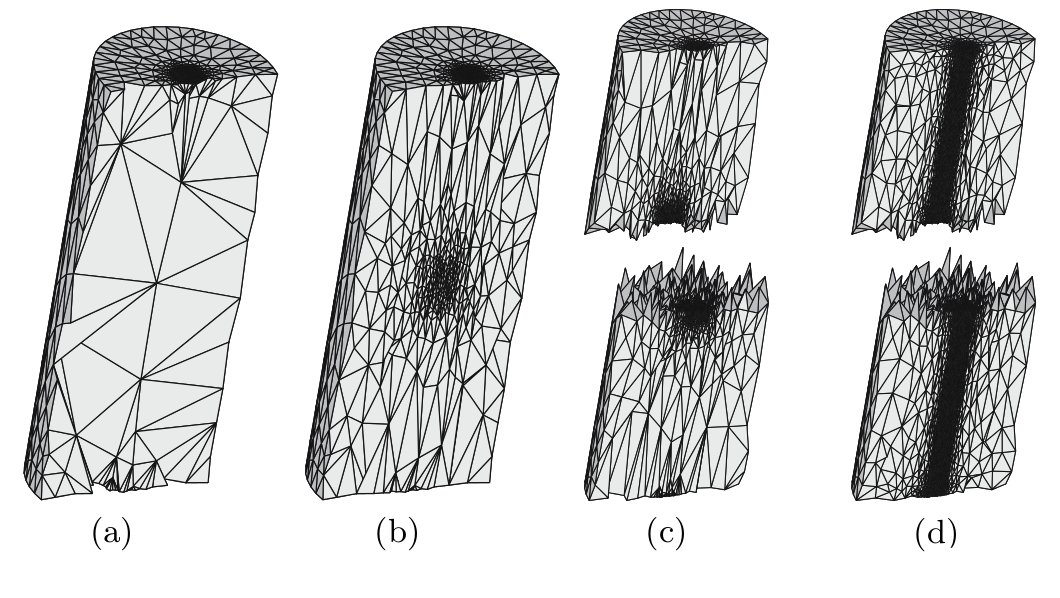
\includegraphics[width=0.8\textwidth]{fig/glut08_2.jpg}
     \caption{Passos da técnica baseada na malha volumétrica grosseira. (a) malha volumétrica grosseira; (b) refinamento da seção transversal; (c) seção transversal; (d) malha final \cite{bib:Glut08}.}
     \label{fig:glut08_2}
 \end{figure}


Esta técnica depende muito da geometria da entrada já que são utilizadas informações da \textit{bounding box} dessa entrada. Isso afeta diretamente a criação dos planos de corte, e por consequência, a malha gerada ao final. Uma das motivações deste trabalho é evitar a criação de subdomínios baseados nos eixos de inércia, pois, segundo o autor, os  resultados não são bons.

\section{Considerações Finais}


As técnicas que foram discutidas neste capítulo, em geral, apresentam bons resultados, mas a estimativa de carga na maioria deles é inexistente ou apenas uma métrica para contagem. Sem uma boa estimativa de carga, o balanceamento de carga pode ser um problema, fazendo o desempenho do algoritmo paralelo cair. A forma mais comum adotada pelos trabalhos é de realizar várias subdivisões até que a quantidade de subdomínios criados sejam maior que a quantidade de processadores disponíveis, com isso a falta de estimativa de carga é contornada.

A forma com que os cortes são posicionados nessas técnicas dependem bastante do formato do objeto de entrada. Além disso, algumas técnicas necessitam de intervenção de um usuário, ou seja, o processo de geração da malha não é totalmente automático. Uma boa abordagem de balanceamento e de decomposição de domínio é essencial para algoritmos de subdivisão de domínios, caso contrário, o tempo para geração de malha pode ser prejudicado e a qualidade da malha ser afetada.
